\part{Part 1: Physics}

\chapterimage{chapter_head_2.pdf} % Chapter heading image

\chapter{Conservation Laws}
Some of the most powerful tools in classical mechanics, including fluid mechanics, are conservation laws. Arising from the profound physical insights of Newton, Leibniz, and others, these laws ensure that the total amount of certain physical quantities within a volume are conserved. For example, conservation of mass ensures that the total mass of a system remains constant, conservation of momentum ensures that the total momentum of a system remains constant, and conservation of energy ensures that the total energy of a system remains constant. While these concepts can be applied by a high-school student for simple systems, such as elastic/inelastic collisions between particles, their application to fluid mechanics is less trivial. Nevertheless, the fundamental concepts of conservation of mass, momentum, and energy still apply to fluids just as well as they do to individual particles, it is only the mathematics that becomes more complex. It is expected that students reading this book have already taken an undergraduate course in fluid mechanics and are familiar with conservation laws. Nevertheless, this chapter reviews these concepts for completeness, and to establish the notation used in the rest of the book. Some other useful references include~\cite{whiteFluidMechanics2015, hirschNumericalComputationInternal2007a, munsonFluidMechanics2013a}.

\section{Reynolds Transport Theorem}\index{Reynolds Transport Theorem}
Before tackling conservation of mass, momentum, and energy in their entirety, we will first consider an arbitrary conserved {\it extensive} quantity $U_{System} = U_{System}(t)$ of a moving system of fluid, which has a related quantity per unit volume $u = u(\vec{x},t)$, where $\vec{x}$ and $t$ are the spatial coordinate and time, respectively. For example, if the extensive property is mass, then the volumetric property is mass per unit volume, or density. We start by imagining a stationary control volume (CV) such as the one in Figure~\ref{fig:reynolds_transport_volume}, denoted by $\Omega$, that is the same shape as the fluid system at some time $t$. We also denote the surface of this volume by $S$ and the outward pointing normal vector on this surface by $\hat{n}$. After some amount of time $dt$, we can imagine that the initial system of fluid embedded within the control volume will move to a deformed position and shape at $t + dt$, while the control volume remains fixed by definition. In this manner, the fluid contained by the system will be equal to that of the control volume at time $t$, plus any incoming or outgoing fluid due to the motion of the system boundaries as it travels with the flow.
\begin{figure}[htbp]
	\centering
	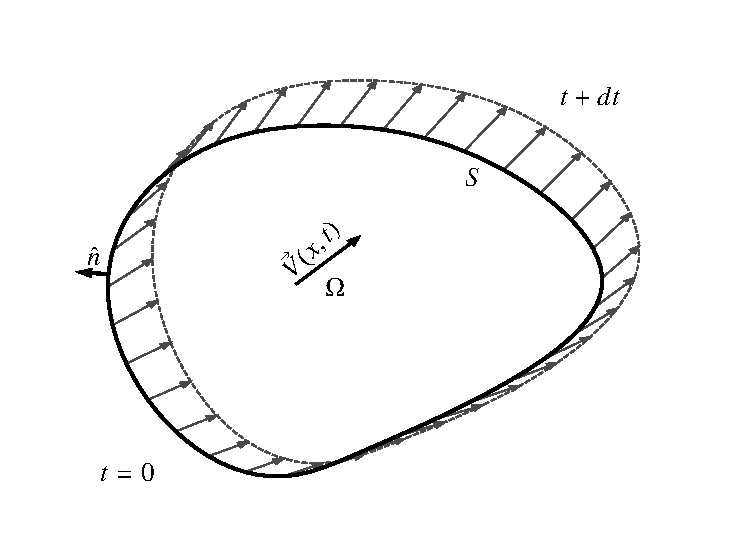
\includegraphics[width=0.5\linewidth]{Pictures/reytrans_volume}
	\caption{Arbitrary flow pattern on an arbitrary volume}
	\label{fig:reynolds_transport_volume}
\end{figure}

Looking at Figure \ref{fig:reynolds_transport_volume}, there are two ways that $U_{System}$ will change with time. Either via a change of $U_{CV}$ within the control volume it overlaps with, or by some amount of the conserved quantity crossing the boundary of the system as it moves. We start by getting the total amount within the control volume $U_{CV}(t)$ by simply adding up, or integrating, $u$ over it. This can be written as
\begin{equation}
	\label{eqn:totalcons}
	U_{CV}(t) = \int_\Omega u d\vec{x},
\end{equation}
noticing that the dependence on space is lost after integration. The time derivative of this is associated with the rate of change of the conserved variable within the control volume itself
\begin{equation}
	\label{eqn:totalcons}
	\frac{dU_{CV}}{dt} = \frac{d}{dt}\int_\Omega u d\vec{x}.
\end{equation}
The second term to be addressed is the change in $U_{System}$ due to the fluid crossing its boundaries.

As noted previously, the second way for $U_{System}$ to change with time is by fluid crossing the surface $S$ as the fluid system advances to $t+dt$. In order for fluid to cross the surface, it must be moving {\it normal} to it, otherwise, it will just move along the surface and not enter the control volume. Hence, we can get the velocity component normal to the surface at any point via the normal vector. Then we can get the total amount of $u$ crossing the surface $S$ by adding up, or integrating, the normal flux at every point on the surface
\begin{equation}
	\label{eqn:totalflux}
	F(t) = \oint_S u (\vec{v} \cdot \hat{n}) ds,
\end{equation}
where $F = F(t)$ is the total rate the conserved quantity $U$ enters/leaves the control volume across the surface.

To create our conservation law, we combine the concepts in Equations \ref{eqn:totalcons} and \ref{eqn:totalflux}. We note that the rate of change of the total amount of the conserved variable within the system $U_{System}$ is equal to the rate at which the conserved variable changes within the control volume and the rate it enters/leaves across the surface of the system. Mathematically, this can be written as
\begin{equation}
	\frac{dU_{System}}{dt} = \frac{d}{dt}\int_\Omega u d\vec{x} + \oint_S u (\vec{v} \cdot \hat{n}) ds,
\end{equation}
noting that the positive in front of the surface term is due to our normal vector being outward pointing. Known as Reynolds Transport Theorem, this will be the foundation for deriving our conservation of mass, momentum, and energy equations for fluid flows.

\chapter{The Navier Stokes Equations} \label{ch:navier_stokes}

\section{Integral Form}\index{Integral Form}
\subsection{Conservation of Mass}
When considering the mass $m = m(t)$ of our system, the mass per unit volume is the density, denoted by $\rho = \rho(\vec{x},t)$. Since the total mass must be conserved, the internal change within the control volume must equal the rate it leaves/enters over $S$. Hence,
\begin{equation}
	\frac{dm}{dt} = \frac{d}{dt}\int_\Omega \rho d\vec{x} + \oint_S \rho \vec{v} \cdot \hat{n} ds = 0,
\end{equation}
and conservation of mass can be written as
\begin{eqBox}
\begin{equation}
	\frac{d}{dt}\int_\Omega \rho d\vec{x} + \oint_S \rho \vec{v} \cdot \hat{n} ds = 0.
\end{equation}
\end{eqBox}

\subsection{Conservation of Momentum}
From Newton's second-law, we know that the time rate of change of the total momentum of the system is equal to the sum of all forces acting on it. Hence
\begin{equation}
	\sum \vec{F} = \frac{d(m \vec{v})}{dt},
\end{equation}
where the product $m \vec{v}$ is the total momentum of the system. Noting that the momentum per unit volume is $\rho \vec{v}$, and using Reynolds transport theorem, we obtain
\begin{equation}
	 \frac{d}{dt}\int_\Omega \rho \vec{v} d\vec{x} + \oint_S \rho \vec{v} (\vec{v} \cdot \hat{n}) ds = \sum \vec{F},
\end{equation}
which requires knowledge of the forces that will act on the system at any given time, which can be split into surface and body terms. In the current context, only surface terms are considered and body terms, such as gravitational forces, are neglected.

The first of the surface forces is due to the pressure surrounding the system. Since pressure acts normal to a surface, the total pressure force $\vec{F_P}$ can be obtained via integration along the surface. Hence,
\begin{equation}
	\vec{F_P} = \oint_S -p\hat{n} ds,
\end{equation}
where $p$ is the pressure and the negative is included since pressure exerts a force inwards, but our normal vector is defined as outwards. The second set of surface terms is due to the effects of viscosity. To account for these we introduce the Cauchy stress tensor $\tau$, which for Newtonian fluids is~\cite{hirschNumericalComputationInternal2007a}
\begin{equation}
	\label{eqn:cauchytensor}
	\tau = \mu \left(\nabla \vec{v} + \left(\nabla \vec{v} \right)^T \right) - \frac{2}{3} \mu \left(\nabla \cdot \vec{v} \right) \mathbf{I},
\end{equation}
where $\mu$ is the dynamic viscosity and $\mathbf{I}$ is an identity matrix. Whereas pressure acts normal to the control volume surface, viscous effects act parallel to it. Hence, the total viscous force $\vec{F_v}$ can be obtained via integration
\begin{equation}
	\vec{F_v} = \oint_S \tau \cdot \hat{n} ds.
\end{equation}
With the inviscid and forces determined, conservation of momentum can be written as
\begin{equation}
	 \frac{d}{dt}\int_\Omega \rho \vec{v} d\vec{x} + \oint_S \rho \vec{v} (\vec{v} \cdot \hat{n}) ds = \oint_S -P\hat{n} ds + \oint_S \tau \cdot \hat{n} ds,
\end{equation}
which is commonly written by grouping all of the surface integral terms
\begin{eqBox}
\begin{equation}
	 \frac{d}{dt}\int_\Omega \rho \vec{v} d\vec{x} + \oint_S \left[ \rho \vec{v} \otimes \vec{v} - \sigma \right]\cdot \hat{n} ds =  0,
\end{equation}
\end{eqBox}
where
\begin{equation}
	\sigma = -p \mathbf{I} + \tau.
\end{equation}

\subsection{Conservation of Energy}
From conservation of energy, the rate of change of energy within the system is equal to the rate of heat added to the system less the rate work done by the system on its surroundings. Hence,
\begin{equation}
	\frac{dE}{dt} = \dot{Q}-\dot{W},
\end{equation}
where $E$ is the energy in the system, $\dot{Q}$ is heat rate, and $\dot {W}$ is work rate. In this case, the energy per unit volume is $\rho e$ where 
\begin{equation}
e = c_v T + \frac{1}{2} \vec{v} \cdot \vec{v},
\end{equation} 
is the specific energy, $c_v$ is the specific heat at constant volume, and $T$ is the temperature. Using Reynolds transport theorem, we have
\begin{equation}
\frac{d}{dt}\int_\Omega \rho e d\vec{x} + \oint_S \rho e (\vec{v} \cdot \hat{n}) ds = \dot{Q}-\dot{W}.
\end{equation}

Since body forces have been neglected, the work done by the system on its surroundings is due to only surface forces. The work done by pressure $\dot{W}_p$ is due to the product of the pressure force, which acts normal to the boundary, and the velocity of the boundary in the normal direction. Hence,
\begin{equation}
	\dot{W}_p = \oint_S p(\vec{v} \cdot \hat{n}) ds.
\end{equation}
Similarly, the work done by viscous forces, $\dot{W}_v$, is due to the product of the viscous stresses and the velocity on the surface. Hence, 
\begin{equation}
	\dot{W}_v = -\oint_S \tau \cdot \vec{v} ds.
\end{equation}
In the above equations, note that, by convention, work is defined as from the system to the surroundings.

The second way that energy can be transferred to the system across the surfaces is thermal diffusion via conduction, denoted by $\dot{Q}$. From Fourier's law, the heat diffused at any point in the fluid is
\begin{equation}
	\vec{q} = -k \nabla T,
\end{equation}
where $k$ is the thermal conductivity of the fluid. Again, only the component of heat that is diffused normal to the surface of the control volume will actually enter it. Hence, the heat added to the system is
\begin{equation}
	\dot{Q} = \oint_S k \nabla T \cdot \hat{n} ds,
\end{equation}
again noting that heat transfer is defined as from the surroundings to the system.

From the work and heat transfer terms, we can now write an expression for conservation of energy
\begin{equation}
\frac{d}{dt}\int_\Omega \rho e d\vec{x} + \oint_S \rho e (\vec{v} \cdot \hat{n}) ds = \oint_S k \nabla T \cdot \hat{n} ds - \oint_S p(\vec{v} \cdot \hat{n}) ds + \oint_S (\tau \cdot \vec{v})\cdot \hat{n} ds.
\end{equation}
Similar to the momentum equation, this is often written more compactly as
\begin{eqBox}
\begin{equation}
\frac{d}{dt}\int_\Omega \rho e d\vec{x} + \oint_S \left[ \rho e \vec{v} + p\vec{v} - \tau \cdot \vec{v} - k \nabla T \right] \cdot \hat{n} ds = 0.
\end{equation}
\end{eqBox}

\subsection{Compact Integral Form}
One might notice that the conservation of mass, momentum, and energy equations derived in the previous sections all have a similar form. They include a time derivative of the conserved variable integrated over the control volume, and a surface integral term of fluxes across the control volume surface. Commonly these equations are compacted into a vector of conserved quantities
\begin{align}
	\vec{w} &= \begin{bmatrix}
		\rho \\
	    \rho \vec{v} \\
	    \rho e
	\end{bmatrix},
\end{align}
a vector of inviscid fluxes
\begin{align}
	\vec{F}_{inv} &= \begin{bmatrix}
		\rho \vec{v} \\
	    \rho \vec{v} \otimes \vec{v} + p \mathbf{I} \\
	    \rho e \vec{v} + p\vec{v}
	\end{bmatrix},
\end{align}
and viscous fluxes
\begin{align}
	\vec{F}_{vis} &= \begin{bmatrix}
		0 \\
	    \tau \\
	    \tau \cdot \vec{v} - \vec{q}
	\end{bmatrix}.
\end{align}
This allows the integral form of the Navier-Stokes equations to be written compactly as
\begin{eqBox}
\begin{equation}
\label{eqn:compactintegral}
\frac{d}{dt}\int_\Omega \vec{w} d\vec{x} + \oint_S \left[\vec{F}_{inv} - \vec{F}_{vis}\right] \cdot \hat{n} ds = 0.
\end{equation}
\end{eqBox}


\section{Divergence Form}\index{Divergence Form}
Looking back at the previous section, we note that Equation \ref{eqn:totalcons} is a general conservation law for a finite control volume. In some contexts, specifically when using the finite-volume method that will be introduced later, this {\it integral form} of the governing equations is used. However, other approaches in CFD use a nearly equivalent {\it divergence form} of Equation \ref{eqn:totalcons}. To derive this form, we rely on the divergence theorem, also known as Gauss theorem.
\begin{theorem}[Divergence Theorem]
The divergence theorem states that integrals of the following form are equivalent for a continuously differentiable vector field $\vec{F}$
\begin{align}
\int_\Omega \nabla \cdot \vec{F} d\vec{x} = \oint_S \vec{F} \cdot \hat{n} ds,
\end{align}
which allows us to transform volume integrals into surface integrals, or the reverse.
\end{theorem}

\subsection{Conservation of Mass}
Starting from the integral form of conservation of mass and applying the divergence theorem to the surface term, we obtain
\begin{equation}
	\frac{d}{dt}\int_\Omega \rho d\vec{x} + \int_\Omega \nabla \cdot (\rho \vec{v}) d\vec{x} = 0.
\end{equation}
Since integration and differentiation commute, we can bring the time derivative inside of the first integral
\begin{equation}
	\int_\Omega \frac{\partial \rho}{\partial t} d\vec{x} + \int_\Omega \nabla \cdot (\rho \vec{v}) d\vec{x} = 0.
\end{equation}
and noticing that the bounds of both integrals are the same
\begin{equation}
	\int_\Omega \left( \frac{\partial \rho}{\partial t} + \nabla \cdot (\rho \vec{v}) \right) d\vec{x} = 0.
\end{equation}
In order for this equation to be valid, other than in trivial cases, we require that the integrand be identically zero. Hence, conservation of mass in divergence form can be written as
\begin{eqBox}
\begin{equation}
	\frac{\partial \rho}{\partial t} + \nabla \cdot (\rho \vec{v}) = 0.
\end{equation}
\end{eqBox}
It is interesting to note that we have effectively converted a problem involving surface and volume integrals, into a differential form that requires computing derivatives.

\begin{remark}
A subtle difference between the two forms of conservation laws is that the integral form applies to control volumes and the divergence form applies at points. This will become important in choosing what form to use for CFD, and will be explored later.
\end{remark}

\subsection{Conservation of Momentum}
Applying the same sets of operations to the integral form of the momentum equation, we can obtain its divergence form
\begin{eqBox}
\begin{equation}
	 \frac{\partial \rho \vec{v}}{\partial t} + \nabla \cdot \left[ \rho \vec{v} \otimes \vec{v} - \sigma \right] =  0.
\end{equation}
\end{eqBox}

\subsection{Conservation of Energy}
Applying the same sets of operations to the integral form of the energy equation, we can obtain its divergence form
\begin{eqBox}
\begin{equation}
\frac{\partial \rho e}{\partial t} + \nabla \cdot \left[ \rho e \vec{v} + p\vec{v} - \tau \cdot \vec{v} - k \nabla T \right] = 0.
\end{equation}
\end{eqBox}

\subsection{Compact Divergence Form}
Considering the compact integral form given in Equation \ref{eqn:compactintegral}, we notice that the divergence theorem can also be applied. Hence, a compact differential form of the Navier-Stokes equations can be obtained
\begin{eqBox}
\begin{equation}
\frac{\partial \vec{w}}{\partial t} + \nabla \cdot \left[\vec{F}_{inv} - \vec{F}_{vis}\right] = 0.
\end{equation}
\end{eqBox}

\chapter{Simplified Systems}

One might notice that the Navier-Stokes equations derived in the previous chapter are a complex system of coupled non-linear partial differential equations. This is not something that sounds particularly easy to solve! Hence, in CFD we often consider {\it simplified} systems of equations first, neglecting or decoupling some of the physical mechanisms that are involved in the full Navier-Stokes equations. This allows us to play with different ideas quickly and with relative ease. Then, once we understand how to solve different parts of these simplified equations, we will combine these ideas later to solve the full Navier-Stokes equations. 

\section{Euler Equations}\index{Euler Equations}
The Euler equations, although they were actually derived prior to Navier-Stokes, can be obtained by simply neglecting viscous effects. Hence, we can ignore physical viscosity and thermal diffusion. While historically the Euler equations were the state-of-the-art in CFD, their lack of viscosity means they are unsuitable for predicting boundary layers. Nevertheless, they are still useful for predicting many flow phenomena, such as shockwaves.

In integral form the Euler equations are
\begin{eqBox}
\begin{equation}
	 \frac{d}{dt}\int_\Omega \rho d\vec{x} + \oint_S \rho \vec{v} \cdot \hat{n} ds = 0,
\end{equation}
\begin{equation}
	\frac{d}{dt}\int_\Omega \rho \vec{v} d\vec{x} + \oint_S \left[ \rho \vec{v} \otimes \vec{v} + p \mathbf{I} \right]\cdot \hat{n} ds =  0,
\end{equation}
\begin{equation}
	\frac{d}{dt}\int_\Omega \rho e d\vec{x} + \oint_S \left[ \rho e \vec{v} + p\vec{v} \right] \cdot \hat{n} ds = 0,
\end{equation}
\end{eqBox}
for conservation of mass, momentum, and energy, respectively. Similarly, in divergence form the Euler equations are
\begin{eqBox}
\begin{equation}
	 \frac{\partial \rho}{\partial t} + \nabla \cdot (\rho \vec{v}) = 0,
\end{equation}
\begin{equation}
	\frac{\partial \rho \vec{v}}{\partial t} + \nabla \cdot \left[ \rho \vec{v} \otimes \vec{v} + p \mathbf{I} \right] =  0,
\end{equation}
\begin{equation}
	\frac{\partial \rho e}{\partial t} + \nabla \cdot \left[ \rho e \vec{v} + p\vec{v} \right] = 0,
\end{equation}
\end{eqBox}
for conservation of mass, momentum, and energy.

\section{Linear Advection}\index{Linear Advection}
Even if we consider the Euler equations, we notice that they are still relatively complex and difficult to solve. In what follows, we will use a set of thought experiments to generate a set of three much simpler equations that will be a starting point for our initial exploration of CFD. To start, we will derive the so-called linear advection equation. We begin our thought experiment by considering a fluid flow that has uniform velocity throughout the domain. Furthermore, we will decouple conservation of mass from the other two conservation laws. 

Now we can imagine that our fluid flow, with constant velocity everywhere such that $\vec{v}(\vec{x},t) = \vec{\alpha}$, has some blob of fluid that is dense relative to the rest of the fluid around it. For example, it could be slightly colder, increasing its density. What should happen to this blob of fluid over time? Well, since the fluid is all moving at the same velocity $\vec{\alpha}$, we would expect the blob of dense fluid to simply move along with the rest of the flow and, hence, the blob should move at velocity $\vec{\alpha}$, as shown in Figure \ref{fig:advection_equation}.

Mathematically, this yields the following integral and differential forms for the linear advection equation by using conservation of mass and replacing the velocity by a constant velocity field $\vec{\alpha}$ and the density by a general scalar $u$ we obtain,
\begin{eqBox}
\begin{equation}
	\frac{d}{dt}\int_\Omega u d\vec{x} + \oint_S (\vec{\alpha}u) \cdot \hat{n} ds = 0,
\end{equation}
and
\begin{equation}
	\frac{\partial u}{\partial t} + \nabla \cdot (\vec{\alpha} u) = 0.
\end{equation}
\end{eqBox}
Furthermore, if we restrict ourselves to one-dimensional problems, we obtain the following integral and differential forms for linear advection
\begin{eqBox}
\begin{equation}
	\frac{d}{dt}\int_\Omega u dx + \alpha \oint_S u \cdot \hat{n} ds = 0,
\end{equation}
and
\begin{equation}
	\frac{\partial u}{\partial t} +  \alpha \frac{\partial u}{\partial x} = 0.
\end{equation}
\end{eqBox}
\begin{figure}[htbp]
	\centering
	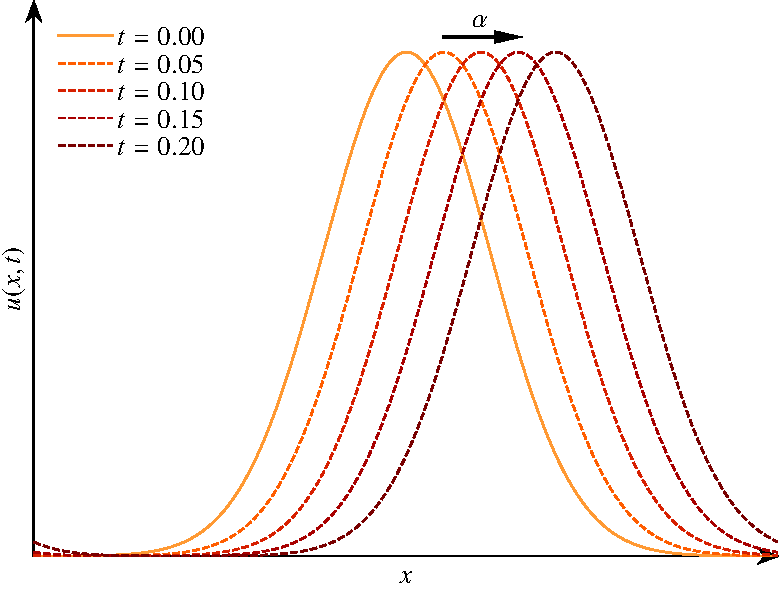
\includegraphics[width=0.65\linewidth]{Pictures/advection_equation}
	\caption{Evolution of a gaussian bump $u(x,0)=\exp\left[-40\left(x-\frac{1}{2}\right)^2\right]$ using the advection equation on $x\in[0,1]$ with velocity $\alpha=1$, and periodic boundary conditions.}
	\label{fig:advection_equation}
\end{figure}

\section{Burgers Equation}\index{Burgers Equation}
Our second simplified system, known as Burgers equation, is useful as a simplified model for compressible flow features such as shocks and expansion fans. To derive Burgers equation, we start with the momentum equation, decoupled from conservation of mass and conservation of energy. Then, neglecting the effects of viscosity and pressure, we replace the momentum with an arbitrary conserved variable $u$, and restrict ourselves to one physical dimension. 

This yields the following integral and differential forms of the Burgers equation
\begin{eqBox}
\begin{equation}
	 \frac{d}{dt}\int_\Omega u dx + \frac{1}{2}\oint_S u^2 \cdot \hat{n} ds =  0,
\end{equation}
and
\begin{equation}
	\frac{\partial u}{\partial t} +  \frac{1}{2} \frac{\partial u^2}{\partial x} = 0,
\end{equation}
\end{eqBox}
noting that the factor of one half is added to the spatial term by convention.

If we consider the divergence form of Burgers' equation, applying the chain rule to the spatial derivative operator yields
\begin{equation}
	\frac{\partial u}{\partial t} +  u \frac{\partial u}{\partial x} = 0.
\end{equation}
We note that this looks remarkably similar to the divergence form of the linear advection equation, also in one dimension. However, the advection velocity $\alpha$, which appears in front of the spatial derivative for linear advection, has instead been replaced by $u$, the value of the solution. Hence, Burgers equation has similar behaviour to linear advection, except the velocity at any point in space is {\it equal} to the value of the solution at that point, rather than being a constant value throughout the domain. An example of this is shown in Figure \ref{fig:burgers_equation}, where the solution at any point moves at a speed equal to its value. This causes the bump to deform, with the forward-moving peak catching up with the slower moving fluid in front of it. This causes the formation of a discontinuity, or shockwave, in the solution on the right hand side of the domain.
\begin{figure}[htbp]
	\centering
	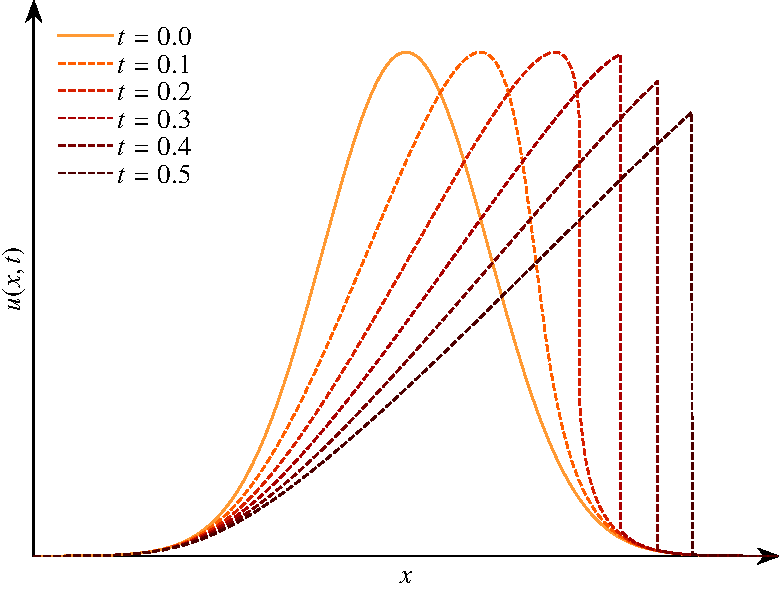
\includegraphics[width=0.65\linewidth]{Pictures/burgers_equation}
	\caption{Evolution of a gaussian bump $u(x,0)=\exp\left[-40\left(x-\frac{1}{2}\right)^2\right]$ using Burgers equation on $x\in[0,1]$.}
	\label{fig:burgers_equation}
\end{figure}
\section{Linear Diffusion}\index{Linear Diffusion}
Our third and final simplified equation, known as linear diffusion, starts again from a simple thought experiment. First, we will consider only the energy equation decoupled from conservation of mass and momentum. We will now imagine that we have a stationary fluid with zero velocity everywhere in the domain. Similar to linear advection, we will consider a flow with some blob of fluid with more energy than the fluid around it. Since all of the fluid is stationary, this extra energy must come in the form of heat. As time goes on, we would expect that this local region of hot fluid would diffuse some of its heat over time to the cold fluid that is adjacent to it. Hence, over time an initially concentrated blob of heat would spread out, until eventually all of the fluid is at the same temperature.

Mathematically, the equation describing this can be obtained by taking $\beta = k/{\rho c_v}$ as a constant scalar and replacing $e$ with a generic scalar $u$. We can then rewrite the energy equation in multiple dimensions as
\begin{eqBox}
\begin{equation}
\frac{d}{dt}\int_\Omega u d\vec{x} + \oint_S \left[ - \beta \nabla u \right] \cdot \hat{n} ds = 0.
\end{equation}
and
\begin{equation}
\frac{\partial u}{\partial t} - \nabla \cdot (\beta \nabla u) = 0,
\end{equation}
\end{eqBox}
in integral and divergence form, respectively. Furthermore, if we restrict ourselves to one dimension we obtain
\begin{eqBox}
\begin{equation}
\frac{d}{dt}\int_\Omega u dx + \oint_S \left[ - \beta  \frac{\partial u}{x} \right] \cdot \hat{n} ds = 0.
\end{equation}
and
\begin{equation}
\frac{\partial u}{\partial t} - \beta \frac{\partial^2 u}{\partial x^2} = 0.
\end{equation}
\end{eqBox}
At this point, it is worth noting that the form of the linear diffusion equation is similar to the linear advection equation, except we are taking the second derivative rather than the first. An example of the evolution of the diffusion equation is shown in Figure \ref{fig:diffusion_equation}, demonstrated that as the solution evolves the concentrated energy is spread out to the surrounding fluid.
\begin{figure}[htbp]
	\centering
	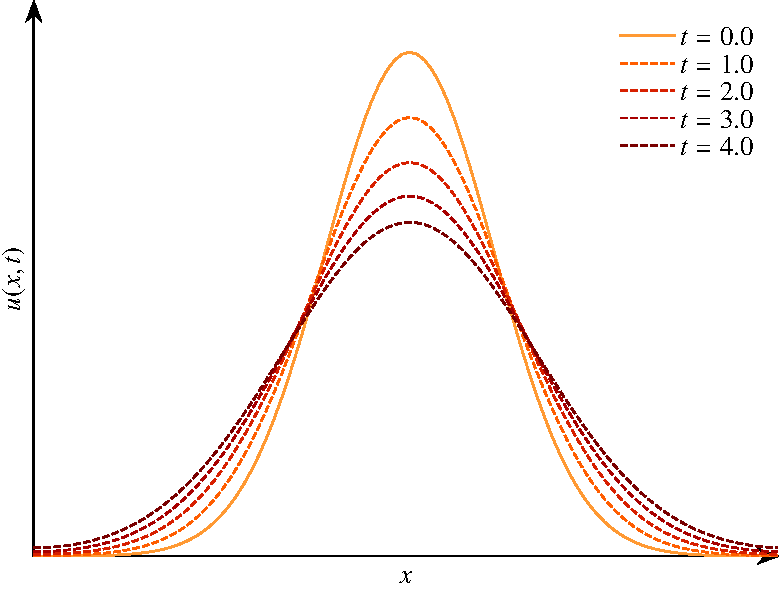
\includegraphics[width=0.65\linewidth]{Pictures/diffusion_equation}
	\caption{Evolution of a gaussian bump $u(x,0)=\exp\left[-40\left(x-\frac{1}{2}\right)^2\right]$ using the linear diffusion equation on $x\in[0,1]$.}
	\label{fig:diffusion_equation}
\end{figure}
\section{PDE Classification}\index{PDE Classification}
In the previous sections, we have introduced several different partial differential equations. From the context of the Navier-Stokes equations, these include conservation of mass, momentum, and energy, which we have then simplified into the Euler, linear advection, Burgers, and linear diffusion equations. As we will see in later sections, not all numerical approaches work well for all partial differential equations, and it is often useful to classify them based on their properties and behaviour.

\subsection{First Order Equations}
First order partial differential equations take the form
\begin{equation}
	A \frac{\partial u}{\partial x} + B \frac{\partial u}{\partial y} = F(x,y,u).
\end{equation}
Note that the $x$ and $y$ dimensions here need not be only space, this is just a general form. Hence, the linear advection equation is also of this form, since both of its derivatives are first order in both space and time. These are always {\it hyperbolic} in nature, and as a result, they exhibit wavelike solutions. This means that information travels in a particular defined direction, as was demonstrated for the linear advection and Burgers equations.

\subsection{Second Order Equations}
Second order partial differential equations take the form
\begin{equation}
	A \frac{\partial^2 u}{\partial x^2} + B \frac{\partial^2 u}{\partial x \partial y} + C \frac{\partial^2 u}{\partial y^2} = F(x,y,u,\frac{\partial u}{\partial x},\frac{\partial u}{\partial y}).
\end{equation}
Depending on the values of $A$, $B$, and $C$, these type of equations will exhibit different behaviour.

\subsubsection{$B^2-4AC > 0$}
These are also hyperbolic in nature, and exhibit wave-like solutions.

\subsubsection{$B^2-4AC = 0$}
These are parabolic in nature, and are typically transient diffusion processes.

\subsubsection{$B^2-4AC < 0$}
These are elliptic in nature, and are typically steady-state diffusion processes.

If we look at linear advection, it is first order and, therefore hyperbolic. If we look at the linear diffusion equation, we find that it is parabolic. Hence, we expect that the numerical behaviour of these two different problems will be quite different. A few other examples include the classical wave equation
\begin{equation}
	\frac{\partial^2 u}{\partial t^2} - \alpha\frac{\partial^2 u}{\partial t^2} = 0,
\end{equation}
which is hyperbolic and should have similar behaviour to the linear advection equation. Also, a steady-state two dimensional diffusion problem has the form
\begin{equation}
	\frac{\partial^2 u}{\partial x^2} + \frac{\partial^2 u}{\partial t^2} = 0,
\end{equation}
which is elliptic, and will typically require a different solution strategy.

The above is a relatively simple classification, but when confronted with a new type of partial differential equation, it is very useful to identify its classification to see if its behaviour is similar to another well-known system. In addition, in many applications the $A$, $B$, and $C$ coefficients can be a function of space, time, or a non-linear function of the solution. Hence, the behaviour of the system can change from one type to another as the solution evolves. In this case, a particularly robust numerical approach is required.
 
\chapter{Turbulence}
One of the most challenging aspects of CFD is the prevalence of turbulent flows. While it may not be immediately apparent from the Navier-Stokes equations defined earlier, they can encode solutions with chaotic, unsteady, three-dimensional flow features. In this section, we will discuss what is meant by turbulent flow, the nature of chaos, how it arises in the governing equations, and consequences for how we handle turbulent flows in CFD. Then, we will introduce an approach for approximating the effects of turbulence, and several popular models for doing so. Some other useful references for this section include~\cite{pope2001turbulent, davidson2015turbulence}.

\section{Turbulence Theory}
The fundamental characteristic of turbulence is that it is {\it chaotic}. Hence, it encodes unsteady three-dimensional fluid flow with chaotic fluctuations in velocity, density, and pressure. These fluctuations typically exist over a wide range of length and time scales. Another important feature of turbulence, and a fundamental property of chaotic systems, is that it is highly sensitive to initial conditions. Furthermore, it is well known that chaotic behaviour only arises in {\it non-linear systems}. In our exploration of turbulence we will first start with a simple chaotic system, and then we will extrapolate some of the properties of these systems to the types of behaviour we observe in fluid flows.

\subsection{Introduction to Chaos}
As an introduction to chaos, we will consider the relatively simple logistic map, which is built from the non-linear logistic function~\cite{strogatz2018nonlinear}
\begin{equation}
	x_{n+1} = ax_n(1-x_n),
	\label{eq:logistic_function}
\end{equation}
where $x_n$ is the current value, $x_{n+1}$ is the next value, and $a$ is a scalar that governs the behaviour of the system. A relatively simple analogy/application of the logistic equation is the growth/decay of a population of animals. In this case $x_n$ would be the current population, $x_{n+1}$ is next years population, and $a$ is responsible for controlling the birth/death rate of the animals in any given year based on the current population. The first thing to notice is that this equation is incredibly simple, yet under certain conditions it encodes infinitely complex chaotic behaviour, and the behaviour of the system is governed by the choice of $a$.

\subsubsection{$a\leq 3$}
In this case, regardless of the initial value $x_0$, the solution converges to one of two fixed points, either $x=0$, or $x=(a-1)/a$. In the context of a population prediction, this means that either all of the animals die, or the population converges to a constant value.

\subsubsection{$ 3 < a \leq 1 + \sqrt{6}$}
In this case, the system rapidly flips back and forth between two different values, referred to as a {\it two-cycle}. Regardless of the initial condition, the system will converge to one of these values, and then flip alternating back and forth between them. The transition from the initial fixed-point solution to this two-cycle is referred to as a {\it bifurcation}. From a population perspective, this means alternating years of famine, where many animals die, and feast, where many animals are born.

\subsubsection{$1 + \sqrt{6} < a \leq 3.54\hdots$}
In this case, a second bifurcation occurs, and the solution oscillates between four possible solutions. This is referred to as a {\it period doubling}. As a consequence, the population will be a more complex cycle of feast and famine.

\subsubsection{$\leq 3.54\hdots < a \leq 3.57\hdots$}
Beyond $a = 3.54\hdots$, additional bifurcations and period doublings occur, with the population now oscillating between an ever-growing number of possible values. By $a = 3.57\hdots$, an infinite number of bifurcations occurs. 

\subsubsection{$3.57\hdots < a $}
Beyond $a = 3.57\hdots$, the entire concept of a cycle breaks down, and all possible solution can be found within the range. The solution traverses chaotically and little structure is observed in its behaviour. 

\begin{figure}[htbp]
	\centering
	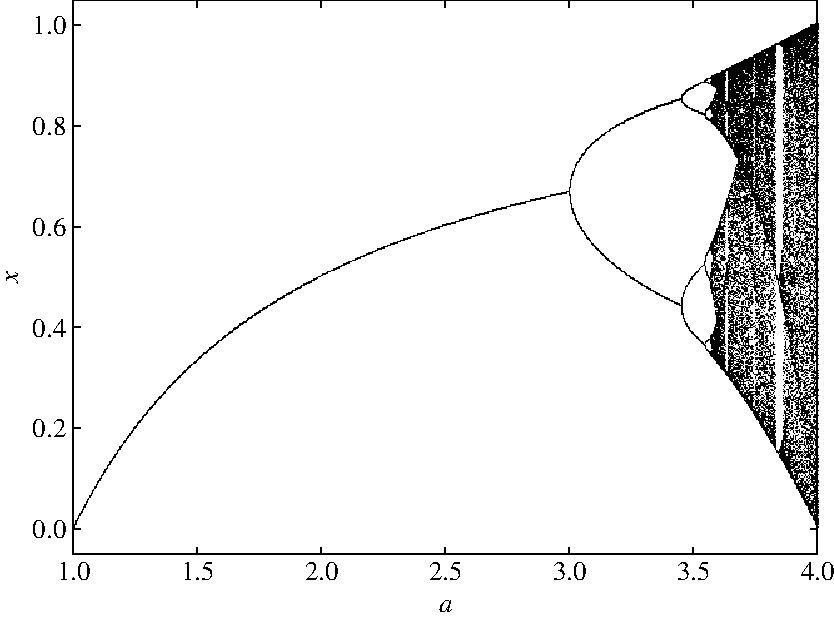
\includegraphics[width=0.65\linewidth]{Pictures/logistic_map}
	\caption{Logistic map for $a\in[1,4]$}
	\label{fig:logistic_map}
\end{figure}
The complete behaviour of Equation~\ref{eq:logistic_function} can be observed in Figure~\ref{fig:logistic_map} for a range of values of $a$ in the range $a\in[1,4]$. An interesting thought experiment is to consider what happens to our system when we start with some initial guess $x_0$, and some perturbed initial guess $x_0 + \epsilon$, where $\epsilon$ is a small number. In the case of small values of $a$ both of these solution converge to the same fixed point. However, as $a$ gets larger, this predictability starts to break down. Eventually, with a large value of $a$, and given enough iterations, the two solutions will diverge from one another, and it will be impossible to discern that they had almost the exact same initial condition. Hence, with certain choices of $a$ the logistic equations is chaotic, resulting in complex behaviour and extreme sensitivity to initial conditions. Furthermore, this implies that there is an {\it irreversible} nature to chaotic systems, that is, given a final solution, it is not possible to determine with any certainty what the initial condition was, because very similar initial conditions yield completely different final solutions.
\begin{jupyternote}
	Check out the Chaos Jupyter notebook \href{\binderurl}{\underline{here}}. You can also download the files from the Gitlab repository \href{\repourl}{\underline{here}}.
\end{jupyternote}

\subsection{Chaos and Navier-Stokes}
In the above, we have demonstrated a couple of properties of chaos. It arises in non-linear systems, and it is generally irreversible due to an extreme sensitivity to initial conditions. For simplicity, we will explore the connection between the Navier-Stokes equations and chaos, in the form of turbulence, via the incompressible Navier-Stokes equations. This can also be readily extended to the compressible Navier-Stokes equations at the readers' initiative.

In the case of incompressible flow, the Navier-Stokes equations reduce to the continuity equation
\begin{equation}
	\nabla \cdot \vec{v} = 0,
\end{equation}
and the momentum equation
\begin{equation}
	\frac{\partial \vec{v}}{\partial t} + \left(\vec{v} \cdot \nabla \right)\vec{v} - \nu \nabla^2 \vec{u} = 0,
\end{equation}
where $\nu$ is the kinematic viscosity. Starting with conservation of mass, we note that this is a linear equation and, hence, it cannot be responsible for the chaotic nature of turbulence, which requires a non-linear system as previously noted. This allows us to quickly narrow in on the momentum equation as the responsible part of the system. In this case, we note that the non-linearity arises in the $\left(\vec{v} \cdot \nabla \right)\vec{v}$ term, which is quadratic in the velocity components. To better understand this, we will consider two limiting cases of inviscid and high viscosity flows.

Starting with the inviscid case, we can neglect the effects of viscosity, yielding the following simplification of the momentum equation
\begin{equation}
	\frac{\partial \vec{v}}{\partial t} + \left(\vec{v} \cdot \nabla \right)\vec{v} = 0,
\end{equation}
which is the momentum component of the incompressible Euler equations. This is obviously still a non-linear equation, since we have not eliminated the convection term. We can now ask ourselves if this inviscid flow can permit chaotic solutions. Recall that our second requirement for a chaotic system is that it should be irreversible. In order to explore this we will reverse this momentum equation in time by setting $t=-t$ and $\vec{v} = -\vec{v}$, which is equivalent to stopping a solution and then rewinding it in time. Applying these modifications to the forward in time system yields
\begin{equation}
	\frac{\partial (-\vec{v})}{\partial (-t)} + \left((-\vec{v}) \cdot \nabla \right)(-\vec{v}) = 0,
\end{equation}
which simply gives us back our original equation
\begin{equation}
	\frac{\partial \vec{v}}{\partial t} + \left(\vec{v} \cdot \nabla \right)\vec{v} = 0.
\end{equation}
Hence, the incompressible Euler equations are completely time reversible and, hence, cannot permit chaotic solutions. Therefore, we need viscosity to enable turbulence.
\begin{remark}
Careful consideration should be used when extrapolating these conclusions to the compressible Euler equations. In that case, irreversibility can arise across shockwaves, which increase entropy. Hence, turbulence can be observed with the compressible Euler equations in some cases.
\end{remark}

Now, let's explore the alternative of a purely viscous flow, which is the limit that viscosity goes to extremely large values. This yields the following simplification of the momentum equation
\begin{equation}
	\frac{\partial \vec{v}}{\partial t} - \nu \nabla^2 \vec{u} = 0,
\end{equation}
which is a linear equation in velocity. Hence, in the limit of large viscosities, the system of equations becomes linear and can no longer permit chaotic solutions.
\begin{figure}[tbp]
	\centering
	\begin{subfigure}[b]{0.40\textwidth}
		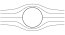
\includegraphics[width=\linewidth]{Pictures/cylinder_1}
		\caption{$Re\approx1$}
	\end{subfigure}
	\begin{subfigure}[b]{0.40\textwidth}
		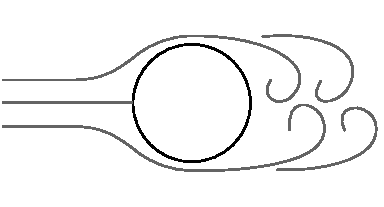
\includegraphics[width=\linewidth]{Pictures/cylinder_2}
		\caption{$Re\approx100$}
	\end{subfigure}
	\begin{subfigure}[b]{0.40\textwidth}
		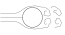
\includegraphics[width=\linewidth]{Pictures/cylinder_3}
		\caption{$Re\approx10^4$}
	\end{subfigure}
	\begin{subfigure}[b]{0.40\textwidth}
		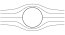
\includegraphics[width=\linewidth]{Pictures/cylinder_1}
		\caption{$Re=\infty$}
	\end{subfigure}
	\caption{Incompressible flow regimes at different Reynolds numbers}
	\label{fig:flow_regimes}
\end{figure}
From the above discussion, it is clear that the momentum equations in the incompressible Navier-Stokes equation are non-linear with respect to the velocity. Furthermore, viscosity is key in determining whether chaotic solutions exist. If there is not enough, the system becomes reversible. In contrast, if there is too much, the system becomes linear. The relative strength of the viscosity is given by the Reynolds number
\begin{equation}
	Re = \frac{UL}{\nu},
\end{equation}
where $U$ and $L$ are the velocity and length scales of the flow, and $\nu$ is the viscosity. Examples of different Reynolds numbers can be observed in Figure~\ref{fig:flow_regimes}. We can note here the similarity of dependence of turbulence on the Reynolds number to the behaviour of the logistic equation on $a$. Typically, turbulent flow is observed for Reynolds numbers of $Re \gtrsim \mathcal{O}(10^3)$. It is important to note that this encompasses the vast majority of flows of engineering interest. Hence, scientists and engineers must routinely deal which turbulence and its chaotic nature.



\subsection{The Energy Cascade}
A common misconception is that turbulence is {\it random} in nature, which would imply that it has no pattern and is inherently unpredictable in a deterministic sense. However, the very fact that one can derive the Navier-Stokes equations, which are a deterministic model for fluid flow, implies that turbulence is not a random process. Hence, in the lack of detailed measurement techniques, turbulence is often {\it modelled} as random process, but its evolution is truly deterministic in nature. Furthermore, turbulent flows clearly have coherent structures, such as turbulent vortices, that demonstrate and underlying structure within the chaos.
\begin{remark}
We will revisit how to model turbulence stochastically when we introduce the Reynolds Averaged Navier-Stokes (RANS) equations and turbulence models.
\end{remark}

One of the most powerful observations of turbulent flow has to do with the distribution of kinetic energy across different physical scales. When considering turbulent flows, there is typically a wide distribution of length scales and time scale with the largest vortices have a size similar to the physical length scale of the problem of interest, such as an airfoils chord length or the size of a bluff body such as a cylinder. In contrast, the smallest physical scales can be much smaller than the physical length scale of the problem, and there is then a wide range of scales between these two extremes. A fundamental observation related to this is that these turbulent structures, over time, tend to break up into multiple smaller structures. A consequence of this is that kinetic energy gradually gets transferred from large-scale structures down to smaller-scale structures and so on, referred to as the {\it turbulent kinetic energy cascade}, which can be observed in Figure~\ref{fig:energy_cascade}.
\begin{figure}[tbp]
	\centering
	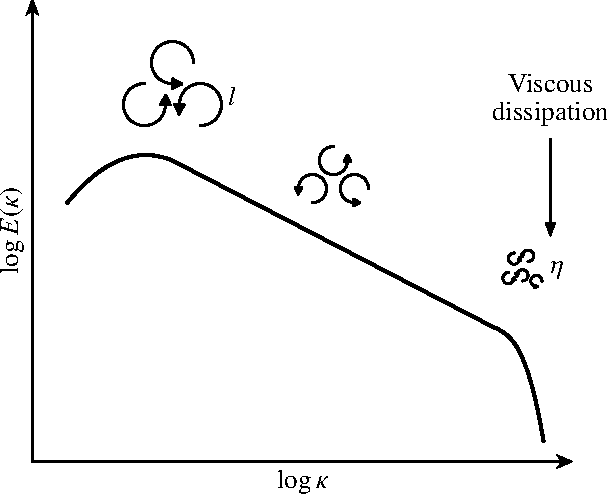
\includegraphics[width=0.5\linewidth]{Pictures/energy_cascade}
	\caption{Turbulent kinetic energy cascade}
	\label{fig:energy_cascade}
\end{figure}

To better understand this, we will define $l$ as the length scale of the largest scale vortices, and $u$ as their velocity scale. Similarly, we will define $\eta$ as the length scale of the smallest scale vortices and $v$ as their velocity scale. For the large scale vortical structures, they will complete a revolution, or turnover time, in approximately
\begin{equation}
	t \sim \frac{l}{u}.
\end{equation}
In experiments, it is observed that a turbulent structure tends to break up within a small number of eddy turnover times, regardless of its size. Hence, the rate at which kinetic energy gets transferred from the largest scales is
\begin{equation}
	\Pi \sim \frac{u^2}{t},
\end{equation}
which expands to 
\begin{equation}
	\Pi \sim \frac{u^3}{l}.
\end{equation}
Hence, if we know the approximate size and velocity of the largest scale turbulent structures, we can estimate the rate at which they transfer energy down to the smaller scales.

Similarly, if we consider the small scale structures, it can be shown via the Navier-Stokes equations that they dissipate their energy via viscous effects into heat at a rate of~\cite{davidson2015turbulence}
\begin{equation}
	\epsilon \sim \nu S_{ij} S_{ij} \sim \nu \frac{v^2}{\eta^2},
\end{equation}
where $\epsilon$ is the rate of kinetic energy dissipation into heat and $S_{ij}$ is the strain rate tensor. Hence, we can also approximate the rate at which kinetic energy ultimately gets turned into heat.

If we consider a quasi steady system, where the rate at which kinetic energy gets introduced to the flow at the large scales has stabilized, then it must balance with the rate at which kinetic energy gets dissipated by the smalles scales. Hence, under these conditions
\begin{equation}
	\Pi = \epsilon,
\end{equation}
which yields
\begin{equation}
	\label{eqn:qpf73j8s}
	\frac{u^3}{l} \sim \nu \frac{v^2}{\eta^2}.
\end{equation}
Considering again the smallest scale structures, we would expect the dissipation due to viscous effects to start to dominate when they are about the same strength as the intertial effects. Hence, at the smallest scales, the kinetic energy is expected to diffuse into heat when
\begin{equation}
	Re = \frac{v \eta}{\nu} \approx 1.
\end{equation}
In conjunction with Equation \ref{eqn:qpf73j8s}, this yields
\begin{eqBox}
\begin{equation}
	\frac{l}{\eta} \sim Re^{3/4}.
\end{equation}
\end{eqBox}
Hence, if we know the Reynolds number of the flow, we can estimate the approximate size of the largest scales relative to the smallest scales, referred to as the scale separation. A similar procedure for the velocity components yields
\begin{eqBox}
\begin{equation}
	\frac{v}{u} \sim Re^{-1/4},
\end{equation}
\end{eqBox}
which can be used to estimate the relative difference in the velocity magnitudes at the largest and smallest scales as well.

Now, let's consider what this means in the context of CFD. If we have an object that we want to simulate flow over, the domain size needs to be at least as large as the object, which would be $l$. Furthermore, if we want to resolve the smallest scale turbulent structures, then the grid resolution must be approximately the same size as the structures, $\eta$. Furthermore, this mesh must be three dimensional. Hence, we can estimate the total number of grid points that would be required from
\begin{equation}
	N \sim \left(Re^{3/4}\right)^3,
\end{equation}
which expands to
\begin{eqBox}
\begin{equation}
	N \sim Re^{9/4},
\end{equation}
\end{eqBox}
where $N$ is the total number of grid points. Hence, as the Reynolds number goes up, the required number of grid points scales extremely rapidly with the Reynolds number. For practical Reynolds numbers above $Re \sim 10^5$, this rapidly becomes intractable on modern high-performance computers. Therefore, if we want to simulate turbulent flows above $Re \sim 10^5$, we simply cannot resolve the large-scale structures and the small-scale structures in their entirety at the same time. The most common solution to this, which will be explored in the following section, is to resolve only the large scale structures and introduce a {\it model} for the effect the small scale structures will have on the large scale structures. This model will not be able to exactly mimic the effects of the small scale structures and, hence, it will introduce some error into our solution of the largest scales.

\section{Reynolds Averaging}
Now that we have briefly introduced chaos and how it relates to the Navier-Stokes equations, it is clear that the study of turbulent flows is indeed challenging. Small changes in the initial conditions may substantially deviate the results. Furthermore, we have demonstrated that the scale separation between the largest and smallest turbulent structures rapidly becomes intractable as the Reynolds number increases. Hence, we commonly require the use of statistical tools to understand its behaviour, which includes averaging operations. One of the most widely used, known as \textit{Reynolds decomposition}, was introduced by Osborne Reynolds~\cite{reynoldsIVDynamicalTheory1895} in 1895. This concept relies on representing any flow property $u(\vec{x},t)$ as the sum of its mean and fluctuating components, such that
\begin{equation}
	u(x,t) = \overline{u(\vec{x})} + u(\vec{x},t)^\prime,
	\label{eq:reynolds_decomp}
\end{equation}
where $\overline{\cdot}$ denotes the averaged term and $^\prime$ the fluctuation.
Turbulent flows can be considered \textit{stationary} if, after averaging, they do not vary in time. Even though the instantaneous fluctuating components will vary, we gain some reproducibility by considering the mean quantities instead. An example could be a wing of an airplane flying at cruise. It is clear that if we measure the velocity at a given point where the flow is turbulent, we will observe fluctuations in the results. However, if these results are \textit{time-averaged}, we will expect to obtain the same value should the experiment be repeated. This type of averaging is defined in an integral sense as
\begin{equation}
	u_T(\vec{x}) = \lim_{\tau\rightarrow\infty} \frac{1}{\tau} \int_{t_0}^{t_0+\tau} u(\vec{x},t)dt,
	\label{eq:time_averaging}
\end{equation}
where $\tau$ is the length of the averaging. For large values of $\tau$, $u_T$ is independent of the initial conditions. A schematic representation can be observed in Figure~\ref{fig:time_averaging}. We observe a constant value given the stationary characteristic of the flow.
\begin{figure}[htbp]
	\centering
	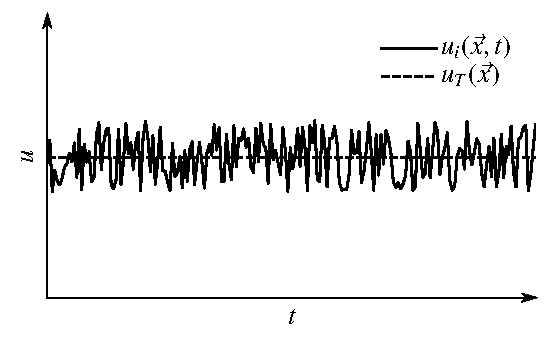
\includegraphics[width=0.6\linewidth]{Pictures/time_averaging}
	\caption{Time averaging of a stationary flow quantity $u(\vec{x},t).$}
	\label{fig:time_averaging}
\end{figure}

\textit{Homogeneous} flows are those whose properties do not vary in any direction. In this case, a \textit{spatial averaging} procedure may be convenient
\begin{equation}
	u_\Omega(t) = \lim_{\Omega\rightarrow\infty} \frac{1}{\Omega}\int_\Omega u(\vec{x},t)dV,
\end{equation}
where $\Omega$ is the volume of the domain. Finally, \textit{ensemble averaging} can be used to obtain mean values using $N$ identical experiments, even if initial and boundary conditions include infinitesimal perturbations. In this type of averaging, the variation on both the spatial and temporal coordinates is maintained. For $N$ experiments, where $N$ is large, we can calculate
\begin{equation}
	u_N(\vec{x},t) = \lim_{N\rightarrow\infty} \frac{1}{N} \sum_{i=1}^N u_i(\vec{x},t),
\end{equation}
where $u_i({\vec{x},t})$ is the result obtained in the $i$-th experiment. An example of ensemble averaging can be seen in Figure~\ref{fig:ensemble_averaging} for non-stationary flows, where we discover a smooth sinusoidal behaviour after $N$ experiments have been performed. 

\begin{figure}[htbp]
	\centering
	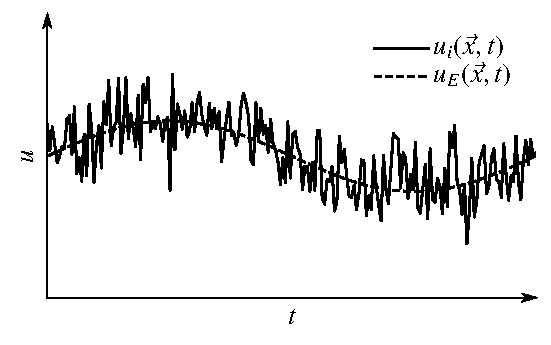
\includegraphics[width=0.6\linewidth]{Pictures/ensemble_averaging}
	\caption{Ensemble averaging results of a non-stationary flow quantity $u(\vec{x},t).$}
	\label{fig:ensemble_averaging}
\end{figure}

In the following section, we will derive the Reynolds Averaged Navier-Stokes equations using the time-averaging operation. Before we dive into the derivation, we will discuss some Reynolds Averaging properties. For a complete explanation of these properties, refer to Wilcox~\cite{wilcox1998turbulence}. 

\subsubsection{Properties of Reynolds Averaging}

Consider a statistically-steady state flow scenario, two flow quantities $u$ and $v$, and constants $\alpha$ and $\beta$.

\begin{itemize}
\item Since the time-averaging process deals with definite integrals, it is a linear operation. Hence, 
\begin{equation}
	\overline{\alpha u + \beta v} = \alpha \overline{u} + \beta \overline{v}.
	\label{eq:reynolds_sum}
\end{equation}
\item The time averaging of integrals and derivatives commute
\begin{equation}
	\overline{\int u dy} = \int \overline{u} dy,  ~~~ \overline{\frac{\partial u}{\partial t}} = \frac{\partial \overline{u}}{\partial t}.
	\label{eq:reynolds_commute}
\end{equation}
\item Any time-averaged fluctuation vanishes, i.e. 
\begin{equation}
	\overline{u^\prime}=0.
	\label{eq:reynolds_fluct}
\end{equation}
\item The average of the product of two instantaneous quantities is given by
\begin{equation}
	\overline{uv} = \overline{\bar{u}\bar{v}} + \overline{u^\prime v^\prime}.
	\label{eq:reynolds_prod}
\end{equation}
\item From the aforementioned properties, it can also be shown that
\begin{equation}
	\overline{\overline{u}} = \overline{u}, ~~~ \overline{u^\prime \overline{v}} = 0.
	\label{eq:reynolds_avgfluct}
\end{equation}
\end{itemize}

\subsection{The Reynolds Averaged Navier-Stokes Equations}

The Reynolds-Averaged Navier-Stokes (RANS) equations are especially useful for analysis of time-marching numerical methods involving statistically steady flow problems. These equations have been widely used in the aerospace industry for decades. The idea is to split each of the flow variables into mean and fluctuating components, and then perform time averaging on the governing equations. As a consequence, high-frequency information is removed from the flow via the averaging procedure. The resulting conservation laws describe only the evolution of the mean flow quantities, which are typically sufficient to determine terms of engineering interest, such as the lift and drag coefficients.

In this section, we will derive the RANS equations for incompressible flow, and later for the compressible case. We will then discuss the appearance of the Reynolds stresses as a consequence of time-averaging the non-linear convective terms from the Navier-Stokes equations.

\subsubsection{Incompressible flow}

Consider the incompressible mass conservation law
\begin{equation}
    \nabla\cdot\vec{v} = 0,
\end{equation}
which we rewrite using tensor notation
\begin{equation}
    \frac{\partial v_i}{\partial x_i} = 0,
\end{equation}
where index $i$ indicates summation over all considered directions. We decompose the velocity variable as the sum of mean and fluctuation components
\begin{equation}
    \overline{\frac{\partial }{\partial x_i}\left(\overline{v_i} + v_i^\prime\right)} = 0.
\end{equation}
Since the time-averaging procedure commutes with derivative operators (Equation~\ref{eq:reynolds_commute}),
\begin{equation}
    \label{eq:rans_mass_decomposed}
    \frac{\partial}{\partial x_i} \overline{\left(\overline{v_i} + v_i^\prime\right)} = 0.
\end{equation}
Using Equations~\ref{eq:reynolds_sum} and~\ref{eq:reynolds_fluct},
\begin{eqBox}
\begin{equation}
	\frac{\partial \overline{v_i}}{\partial x_i} = 0,
	\label{eq:rans_continuity}
\end{equation}
\end{eqBox}
where the fluctuating term has vanished. This means that the divergence of each of the terms in Equation~\ref{eq:rans_mass_decomposed} must equal zero. Hence
\begin{equation}
	\frac{\partial v_i^\prime}{\partial x_i} = 0.
	\label{eq:rans_continuity2}
\end{equation}
Next, we consider the momentum equation. Similarly, we split the variables using Reynolds decomposition and then time-average both sides of the equation. The momentum equations can be written using tensor notation
\begin{equation}
    \label{eq:rans_momentum_initial}
    \rho\frac{\partial v_i}{\partial t} + \rho v_j\frac{\partial v_i}{\partial x_j} =
    - \frac{\partial p}{\partial x_i} + \mu \frac{\partial^2 v_i}{\partial x_j^2},
\end{equation}
where $\mu$ is the dynamic viscosity and $\rho=\overline{\rho}$ is constant due to the incompressible condition. We will simplify the derivation beforehand by considering
\begin{equation}
    \frac{\partial \left(v_jv_i\right)}{\partial x_j} = v_j \frac{\partial v_i}{\partial x_j} + v_i \frac{\partial v_j}{\partial x_j},
\end{equation}
where the second term $\partial v_j/\partial x_j$ vanishes according to continuity. Hence, we write
\begin{equation}
    \frac{\partial \left(v_jv_i\right)}{\partial x_j} = v_j \frac{\partial v_i}{\partial x_j},
\end{equation}
which we use to replace the convective term in Equation~\ref{eq:rans_momentum_initial}, such that
\begin{equation}
    \rho\frac{\partial  v_i}{\partial t} + \rho\frac{\partial  v_j v_i}{\partial x_j} =
    - \frac{\partial p}{\partial x_i} + \mu \frac{\partial^2 v_i}{\partial x_j^2}.
\end{equation}
Decomposing the flow variables and time-averaging the resulting equation, we have
\begin{equation}
    \overline{ 
    \rho\frac{\partial  \left(\overline{v_i}+v_i^\prime\right)}{\partial t} 
    + \rho \frac{\partial  \left(\overline{v_j} + v_j^\prime\right)\left(\overline{v_i}+ v_i^\prime\right)}{\partial x_j}} = \overline{
     - \frac{\partial \left(\overline{p}+p^\prime\right)}{\partial x_i} 
    + \mu \frac{\partial^2 \left(\overline{v_i}
    +v_i^\prime\right)}{\partial x_j^2}}.
\end{equation}
By first resolving multiplications and then applying the Reynolds averaging properties, we obtain the RANS equations for incompressible flow
\begin{eqBox}
\begin{equation}
    \rho \frac{\partial \overline{v_i}}{\partial t} 
    + \rho  \frac{\partial}{\partial x_j} \left(\overline{v_j}\overline{v_i} + \overline{v_j^\prime v_i^\prime}\right)
    =- \frac{\partial \overline{p}}{\partial x_i} 
    + \mu \frac{\partial^2 \overline{v_i}}{\partial x_j^2}.
\end{equation}
\end{eqBox}
Recall the stress tensor $\tau_{ij}$ from Chapter 4, which we now rewrite in tensor notation
\begin{equation}
    \tau_{ij} = 2\mu S_{ij},
\end{equation}
where $S_{ij}$ is the strain-rate tensor
\begin{equation}
    S_{ij} = \frac{1}{2}\left(\frac{\partial v_i}{\partial x_j}+\frac{\partial v_j
    }{\partial x_i}\right).
\end{equation}
We may now rewrite the RANS momentum equation in terms of the stresses and rearrange some terms, such that
\begin{eqBox}
\begin{equation}
    \rho \frac{\partial \overline{v_i}}{\partial t} 
    + \rho  \frac{\partial}{\partial x_j} \left(\overline{v_j}\overline{v_i}\right)
    =- \frac{\partial \overline{p}}{\partial x_i} 
	+ \frac{\partial}{\partial x_j} \left(\overline\tau_{ji} - \rho \overline{v_j^\prime v_i^\prime}\right),
	\label{eq:rans_momentum}
\end{equation}
\end{eqBox}
where $\rho \overline{v_j^\prime v_i^\prime}$ is known as the \textit{Reynolds stress}, which we can define as the \textit{Reynolds stress tensor} $\rho\hat\tau_{ij}$, such that
\begin{equation}
	\hat\tau_{ij} = -\overline{v_i^\prime v_j^\prime}.
\end{equation}
Note that the Reynolds stress tensor is symmetric since$\hat\tau_{ij}=\hat\tau_{ji}$. This means that three diagonal components and three off-diagonal components make a total of six independent variables only in $\hat\tau_{ij}$. This number of unknowns rises to ten if we consider the conserved properties of three-dimensional flow, with density as well as one momentum equation in each direction. Clearly, we have an underdetermined system and require additional equations. Later in this chapter, we derive an equation for the Reynolds stresses and discuss some of the consequences that arise from the averaging of the Navier-Stoke equations. We now look at the RANS equations for compressible flow.

\subsubsection{Compressible flow}

In the previous section, we derived the incompressible form of the RANS equations, where the density variations are negligible, i.e $\rho=\overline{\rho}$. In the case of compressible flow, these variations must be taken into account. However, the equations can become very lengthy and complicated if the conventional averaging procedure is used. To visualize this, let us decompose the mass conservation law using the conventional Reynolds decomposition
\begin{equation}
    \frac{\partial}{\partial t} \left(\overline{\rho} + \rho^\prime\right) + \frac{\partial }{\partial x_i} \left[\left(\overline{\rho}+\rho^\prime\right)\left(\overline{v_i}+v_i^\prime\right)\right] = 0,
\end{equation}
which will introduce correlations involving density fluctuations and may complicate the turbulence modelling, i.e.
\begin{equation}
    \frac{\partial \overline{\rho}}{\partial t}  + \frac{\partial }{\partial x_i} \left(\overline \rho \overline{v_i} + \overline{\rho^\prime v^\prime}\right) = 0.
\end{equation}
By performing a density-weighted time-averaging, introduced by Alexandre Favre in 1969, the equations become simpler and the presence of $\rho^\prime$ can be avoided. It is defined by
\begin{equation}
    \tilde{u}=  \frac{1}{\overline{\rho}} \lim_{n\rightarrow\infty} \frac{1}{n}\sum_{\nu=1}^{\nu=n}\left(\rho u\right)^{(\nu)} = \frac{\overline{\rho u}}{\overline{\rho}},
    \label{eqn:favre_definition}
\end{equation}
where $\overline{\cdot}$ represents the conventional time-averaging. Similar to Reynolds decomposition, we consider the flow properties to be the sum of a mean and fluctuating component
\begin{equation}
    u = \tilde{u} + u^{\prime\prime},
\end{equation}
where $\tilde{u}$ is the \textit{Favre mean} and $u^{\prime\prime}$ is the \textit{Favre fluctuation}. Some properties of the Favre averaging are
\begin{align}
    \overline{\tilde{u}} &= \tilde{u},\\
    \overline{\rho u^{\prime\prime}} &= 0, \\
    \overline{u^{\prime\prime}} &= -\overline{\rho^\prime u^\prime}/{\overline{\rho}}, \\ 
    \overline{\rho u v} &= \overline{\rho}\tilde u\tilde v + \overline{\rho u^{\prime\prime}v^{\prime\prime}}. \label{eqn:favre_rhouv}
\end{align}
We note that $\rho$ is the instantaneous density and that the Favre average differs from the Reynolds averaging properties. For instance, $\overline{u^\prime}=0$, whereas $\overline{u^{\prime\prime}}\neq0$. In addition, the conventional Reynolds and Favre averaging are related by
\begin{align}
    \tilde{u} & = \overline{u} + \overline{\frac{\rho^\prime u^\prime}{\overline \rho}}, \\
    u^{\prime\prime} & = u^\prime - \overline{\frac{\rho^\prime u^\prime}{\overline \rho}}.
\end{align}
We now derive the compressible RANS equations, also known as Favre-Averaged Navier-Stokes Equations (FANS). Starting with conservation of mass, by performing time averaging, we have
\begin{eqBox}
\begin{equation}
    \overline{\frac{\partial\rho}{\partial t}} + \overline{\frac{\partial \rho v_i}{\partial x_i}}= 0.
\end{equation}
\end{eqBox}
Since the time-averaging procedure commutes with the derivatives,
\begin{equation}
    \frac{\partial\overline{\rho}}{\partial t} + \frac{\partial \overline{\rho v_i}}{\partial x_i}= 0.
\end{equation}
The first term can then be Favre decomposed and time averaged
\begin{equation}
    \frac{\partial}{\partial t} \overline{\left(\tilde \rho + \rho^{\prime\prime} \right)} 
    = \frac{\partial \overline \rho}{\partial t},
    \label{eqn:favre_singlevariable}
\end{equation}
and the proof is left as a simple exercise to the reader. The second term $\overline{\rho v_i}$ can be computed using the Favre definition in Equation~\ref{eqn:favre_definition}. The averaged mass conservation equation for compressible flows can then be written
\begin{equation}
    \frac{\partial\overline{\rho}}{\partial t} + \frac{\partial \overline{\rho} \tilde v_i}{\partial x_i}= 0.
\end{equation}
Next, we derive the compressible time-averaged momentum equations. Initially, these are given by 
\begin{equation}
    \frac{\partial }{\partial t} \left(\overline{\rho v_i}\right)
    + \frac{\partial}{\partial x_j} \left(\overline{\rho v_j v_i}\right)
    =- \frac{\partial \overline{p}}{\partial x_i} 
    + \mu \frac{\partial^2 }{\partial x_j^2} \left(\overline{v_i}\right).
\end{equation}
The unsteady term can be computed using Equation~\ref{eqn:favre_definition}. We pay special attention to the convective term, which we expand according to Equation~\ref{eqn:favre_rhouv}
\begin{equation}
    \overline{\rho v_j v_i} = \overline{\rho}\tilde v_j\tilde v_i + \overline{\rho v_j^{\prime\prime} v_i^{\prime\prime}}.
\end{equation}
The time-averaged compressible momentum equations can be written
\begin{eqBox}
\begin{equation}
    \frac{\partial }{\partial t} \left(\overline\rho \tilde v_i \right)
    + \frac{\partial}{\partial x_j} \left(\overline\rho \tilde v_j \tilde v_i + \overline{\rho v_i^{\prime\prime}v_j^{\prime\prime}} \right)
    = - \frac{\partial \overline{p}}{\partial x_i} 
	+ \mu \frac{\partial^2 }{\partial x_j^2} \left(\overline{v_i}\right).
\end{equation}
\end{eqBox}
where single-variable terms such as the pressure and diffusive components follow the same procedure described in Equation~\ref{eqn:favre_singlevariable}. Similar to the incompressible case, we rearrange some terms in the equation, such that
\begin{eqBox}
    \begin{equation}
        \frac{\partial }{\partial t} \left(\overline\rho \tilde v_i \right)
        + \frac{\partial}{\partial x_j} \left(\overline\rho \tilde v_j \tilde v_i \right)
        = - \frac{\partial \overline{p}}{\partial x_i} 
		+ \mu \frac{\partial }{\partial x_j} \left(\overline{\tau_{ji}} - \overline{\rho v_i^{\prime\prime}v_j^{\prime\prime}}\right).
	\label{eq:favre_rans}
    \end{equation}
\end{eqBox}
where $-\overline{\rho v_i^{\prime\prime}v_j^{\prime\prime}}$ is the Reynolds stress, which includes the instantaneous density $\rho$, and $\tau_{ij}$ is the viscous stress tensor. As explained in the incompressible section, the resulting system of equations remains underdetermined due to the Reynolds stresses. Obtaining an equation for these stresses turns out to introduce additional unknowns. We now discuss and derive equations for the Reynolds-stress tensor for incompressible flow.

\subsection{The Reynolds Stresses}
The Reynolds stresses for the incompressible case are given by 
\begin{equation}
	\hat \tau_{ij} = -\rho \overline{v_i^{\prime}v_j^{\prime}}.
\end{equation}
We will show in the next section that we can't solve for them directly. However, for now we can understand their influence on the mean flow. Recall the integral form of the Navier-Stokes equations from Chapter~\ref{ch:navier_stokes}, which we rewrite
\begin{equation}
	\frac{d}{dt}\int_\Omega \rho v_i d\Omega + \oint_S \rho v_i \vec{v} \cdot ds = \oint_S -P ds + \oint_S \tau_{ij} ds.
	\label{eq:integral_ns_turbulence}
\end{equation}
The term on the LHS represents the rate of change of momentum. On the right-hand side of Equation~\ref{eq:integral_ns_turbulence}, the first term is responsible for the convection of momentum in and out of the system, followed by the pressure term, and finally the viscous diffusion of momentum. When we apply our time-averaging to this equation, we obtain
\begin{equation}
	\frac{d}{dt}\int_\Omega \rho \overline v_i d\Omega + \oint_S \rho  \overline v_i  \overline{\vec{v}} \cdot ds = \oint_S - \overline P ds + \oint_S  \left(\overline\tau_{ij}-\rho \overline{v_i^{\prime}v_j^{\prime}}\right)ds.
	\label{eq:integral_ns_turbulence_avg}
\end{equation}
Equation~\ref{eq:integral_ns_turbulence_avg} is similar to the time-averaged systems we have derived in the previous section in differential form, such as Equations~\ref{eq:rans_momentum} and~\ref{eq:favre_rans}. Note that the new Reynolds stress term naturally lumps together with the viscous stresses. In fact, the Reynolds stresses are the \textit{turbulent diffusion} of momentum into $\Omega$.

\subsubsection{Example}
Consider laminar and turbulent flow over a plate that is heated, such as that shown in Figure~\ref{fig:heated_plate_flow}. By taking the average of the turbulent case, the resulting profile will resemble that in Figure~\ref{fig:heated_plate_flow_2}. If we now compare the heat transfer between the time-averaged turbulent case and the laminar profile, we will observe much more heat transfer in the time-averaged profile. The reason is due to the energy transported by the turbulent eddies, which after time-averaging looks like extra diffusion. 
\begin{figure}[htbp]
	\centering
	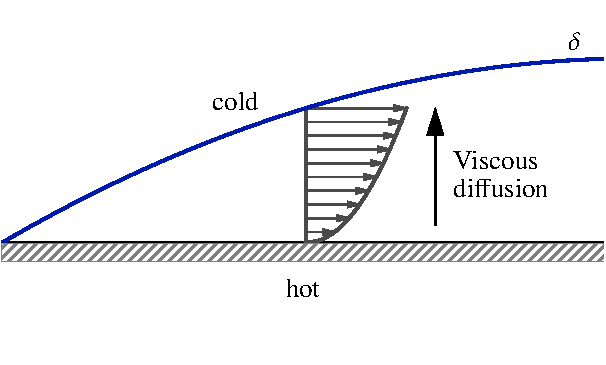
\includegraphics[height=0.25\linewidth]{Pictures/heated_plate_flow_0}~
	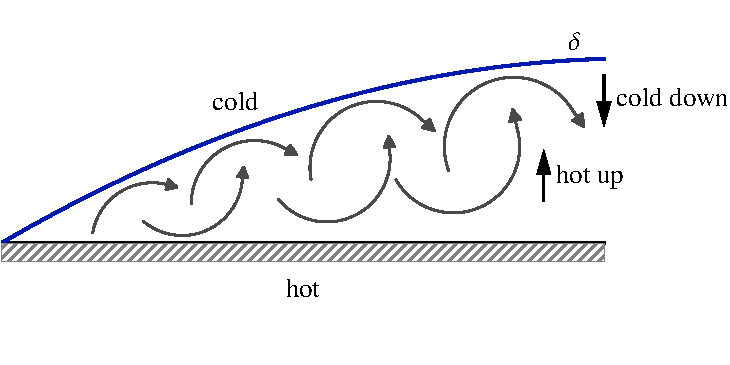
\includegraphics[height=0.25\linewidth]{Pictures/heated_plate_flow_2}
	\caption{Reynolds stresses example}
	\label{fig:heated_plate_flow}
\end{figure}

\begin{figure}[htbp]
	\centering
	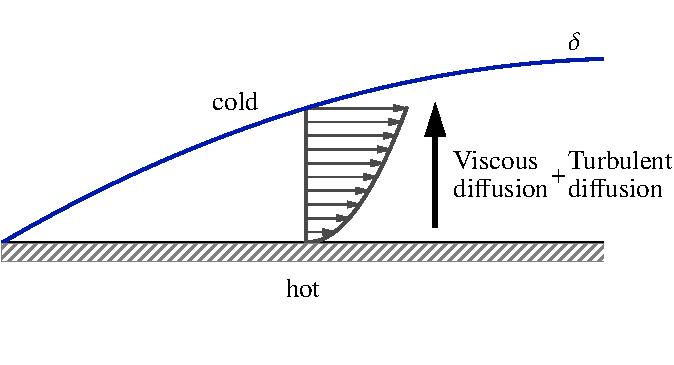
\includegraphics[height=0.25\linewidth]{Pictures/heated_plate_flow_1}
	\caption{Reynolds stresses example}
	\label{fig:heated_plate_flow_2}
\end{figure}

\subsection{The RANS Closure Problem}
As we have previously shown, the Reynolds stresses stem from averaging the convective terms of the Navier-Stokes equations. We now need to find additional equations to solve our system of time-averaged conservation laws. Specifically, we would like to define equations that describe the rate of change of these stresses as we have done for other flow quantities. In this section, we derive the expressions for incompressible flow, however, the derivation can be readily performed for the compressible case considering the Favre averaging procedure. 

Consider the incompressible momentum equation in the $i$-th direction, which we conveniently rewrite 
\begin{equation}
	P(v_i) 
	= \rho \frac{\partial v_i}{\partial t}
	+ \rho v_k\frac{\partial v_i}{\partial x_k}
	+ \frac{\partial p}{\partial x_i} 
	- \mu \frac{\partial^2 v_i}{\partial x_k \partial x_k} =0.
\end{equation}
Since we are looking for a time-averaged symmetric tensor for the Reynolds stresses, we perform the following operation
\begin{equation}
	\overline{v_i^\prime P(v_j) + v_j^\prime P(v_i)}=0.
	\label{eq:reynolds_stresses_1}
\end{equation}
Here, $v_i^\prime$ and $v_j^\prime$ are fluctuation components in the $i$-th and $j$-th direction, respectively. We can compactly rewrite Equation~\ref{eq:reynolds_stresses_1} using
\begin{equation}
	A_{ij} + B_{ij} + C_{ij} + D_{ij} = 0,
\end{equation}
where $A_{ij},~B_{ij},~C_{ij},~D_{ij}$ are the unsteady, convective, pressure and viscous stress tensors from the momentum equations, respectively. For the sake of clarity, we expand each of these terms
\begin{align}
	A_{ij} &= \overline{v_i^\prime\rho\frac{\partial v_j}{\partial t} + v_j^\prime\rho\frac{\partial v_i}{\partial t}},\\
	B_{ij} &= \overline{v_i^\prime\rho v_k\frac{\partial v_j}{\partial x_k} + v_j^\prime\rho v_k\frac{\partial v_i}{\partial x_k}},\\
	C_{ij} &= \overline{v_j^\prime\frac{\partial p}{\partial x_i} + v_i^\prime\frac{\partial p}{\partial x_j}}, \\
	D_{ij} &= \overline{-v_i^\prime\mu\frac{\partial^2 v_j}{\partial x_k\partial x_k}-v_j^\prime\mu\frac{\partial^2 v_i}{\partial x_k\partial x_k}}.
\end{align}
We will now time-average and derive an expression for the Reynolds-stress tensor. Initially, we want to split the instantaneous variables using Reynolds decomposition. Starting with the unsteady term
\begin{equation}
	A_{ij}
	=
	\rho\overline{v_i^\prime \frac{\partial}{\partial t}\left(\overline v_j + v_j^\prime \right)} +
	\rho\overline{v_j^\prime \frac{\partial}{\partial t}\left(\overline v_i + v_{i\vphantom{j}}^\prime \right)}, 
\end{equation}
which we rewrite after solving the products
\begin{equation}
	A_{ij}
	=
	\rho \overline{v_i^\prime\frac{\partial\overline v_j^{\vphantom{\prime}}}{\partial t}} 
	+ \rho \overline{v_i^\prime\frac{\partial v_j^\prime}{\partial t}}
	+ \rho \overline{v_j^\prime\frac{\partial\overline v_{i\vphantom{j}}^{\vphantom{\prime}}}{\partial t}} 
	+ \rho \overline{v_j^\prime\frac{\partial v_{i\vphantom{j}}^\prime}{\partial t}}.
	\label{eq:reystress_A_1}
\end{equation}
Recall from the Reynolds averaging properties in Equation~\ref{eq:reynolds_avgfluct} that the average of the product of a mean and a fluctuating quantity is zero. Hence, we eliminate the first and third terms in Equation~\ref{eq:reystress_A_1}. Furthermore, we apply the product rule to bring fluctuation quantities into the temporal derivative. This yields the time-averaged convective term
\begin{eqBox}
\begin{equation}
	A_{ij}
	= \rho \overline{v_i^\prime\frac{\partial v_j^\prime}{\partial t}}
	+ \rho \overline{v_j^\prime\frac{\partial v_{i\vphantom{j}}^\prime}{\partial t}} 
	= \rho \frac{\partial}{\partial t} \left(\overline{v_i^\prime v_j^\prime}\right).
\end{equation}
\end{eqBox}
Next, we decompose the variables in the convective term
\begin{equation}
	B_{ij} =
	\rho \overline{v_i^\prime \left(\overline v_k+v_{k\vphantom{j}}^\prime\right)\frac{\partial}{\partial x_k}\left(\overline v_j+v_j^\prime\right)}
	+ \rho \overline{v_j^\prime \left(\overline v_k+v_{k\vphantom{j}}^\prime\right)\frac{\partial}{\partial x_k}\left(\overline v_i+v_{i\vphantom{j}}^\prime\right)},
\end{equation} 
whereby solving the products, we obtain
\begin{equation}
	\begin{aligned}
	B_{ij} &=
	\overline{v_i^\prime\overline v_k \frac{\partial\overline v_j^{\vphantom{\prime}}}{\partial x_k} }
	+ \overline{v_i^\prime\overline v_k \frac{\partial v_j^\prime}{\partial x_k} }
	+ \overline{v_i^\prime v_k^\prime \frac{\partial\overline v_j^{\vphantom{\prime}}}{\partial x_k} }
	+ \overline{v_i^\prime v_k^\prime \frac{\partial v_j^\prime}{\partial x_k} } \\
	&+ \overline{v_j^\prime\overline v_k \frac{\partial\overline v_i}{\partial x_k} }
	+ \overline{v_j^\prime\overline v_k \frac{\partial v_i^\prime}{\partial x_k} }
	+ \overline{v_j^\prime v_k^\prime \frac{\partial\overline v_i}{\partial x_k} }
	+ \overline{v_j^\prime v_k^\prime \frac{\partial v_i^\prime}{\partial x_k} }.
	\end{aligned}
	\label{eq:reystress_B_1}
\end{equation}
Note that $\overline{u^\prime \overline v \overline w} = \overline{u^\prime} \overline v \overline w = 0$ as a consequence of Equation~\ref{eq:reynolds_avgfluct}. This way we can clean up Equation~\ref{eq:reystress_B_1} by eliminating the first and fifth terms. In addition, using the product rule for the second and fourth term, we have
\begin{equation}
	\overline{v_i^\prime \overline v_k \frac{\partial v_j^\prime}{\partial x_k} }
	+ \overline{v_j^\prime \overline v_k \frac{\partial v_{i\vphantom{j}}^\prime}{\partial x_k} } 
	= \overline v_k \frac{\partial}{\partial x_k} \left(\overline{v_i^\prime v_j^\prime}\right),
\end{equation}
where $\overline v_k$ is a constant. This yields
\begin{equation}
	B_{ij} = \rho \left[\overline v_k \frac{\partial}{\partial x_k} \left(\overline{v_i^\prime v_j^\prime}\right) 
	+ \overline{v_i^\prime v_k^\prime} \frac{\partial\overline v_j}{\partial x_k}
	+ \overline{v_k^\prime \frac{\partial}{\partial x_k} \left(v_i^\prime v_j^\prime\right)}
	+ \overline{v_j^\prime v_k^\prime}\frac{\partial\overline v_{i\vphantom{j}}}{\partial x_k}\right].
	\label{eq:reystress_B_2}
\end{equation}
We can use the chain rule on the third term of Equation~\ref{eq:reystress_B_2}, such that
\begin{equation}
	\frac{\partial}{\partial x_k} \left(\overline{v_i^\prime v_j^\prime v_k^\prime }\right) 
	= \overline{v_i^\prime v_j^\prime \frac{\partial v_k^\prime}{\partial x_k} } 
	+ \overline{v_k^\prime \frac{\partial\vphantom{v_k^\prime}}{\partial x_k}\left(v_i^\prime v_j^\prime\right)} 
	= \overline{v_k^\prime \frac{\partial\vphantom{v_k^\prime}}{\partial x_k}\left(v_i^\prime v_j^\prime\right)},
\end{equation}
where the first term is zero due to continuity (see Equation~\ref{eq:rans_continuity2}). We can now write the time-averaged convective term of the Reynolds stress equation
\begin{eqBox}
\begin{equation}
	B_{ij} = 
	\overline v_k \frac{\partial}{\partial x_k} \left(\rho \overline{v_i^\prime v_j^\prime}\right) 
	+ \rho \overline{v_i^\prime v_k^\prime}\frac{\partial \overline v_j }{\partial x_k}
	+ \frac{\partial}{\partial x_k} \left(\rho \overline{v_i^\prime v_j^\prime v_k^\prime }\right)
	+ \rho \overline{v_j^\prime v_k^\prime}\frac{\partial \overline v_{i\vphantom{j}}}{\partial x_k}.
\end{equation}
\end{eqBox}
Now, we move on to the pressure term. By splitting the instantaneous quantities, we obtain
\begin{equation}
	C_{ij} = 
	\overline{v_i^\prime \frac{\partial}{\partial x_j} \left(\overline p + p^\prime \right)}
	+ \overline{v_j^\prime \frac{\partial}{\partial x_i} \left(\overline p + p^\prime\right)},
\end{equation}
which after solving the products and cancelling the linear terms yields
\begin{eqBox}
\begin{equation}
	C_{ij} =  
	\overline{v_i^\prime \frac{\partial p^\prime}{\partial x_j}}
	+\overline{v_j^\prime \frac{\partial p^\prime}{\partial x_i}}.
\end{equation}
\end{eqBox}
Finally, we decompose the viscous term
\begin{equation}
	D_{ij} = -\mu \left[ 
	  \overline{v_i^\prime \frac{\partial^2}{\partial x_k\partial x_k} \left(\overline v_j + v_j^\prime\right)}
	+ \overline{v_j^\prime \frac{\partial^2}{\partial x_k\partial x_k} \left(\overline v_i + v_{i\vphantom{j}}^\prime\right)}
	\right],
\end{equation}
whereby solving the products and cancelling corresponding terms yields
\begin{equation}
	D_{ij} = -\mu \left[ 
	  \overline{v_i^\prime \frac{\partial^2 v_j^\prime}{\partial x_k\partial x_k}}
	+ \overline{v_j^\prime \frac{\partial^2 v_{i\vphantom{j}}^\prime }{\partial x_k\partial x_k}}
	\right].
\end{equation}
From the chain rule, we can write
\begin{equation}
	\frac{\partial^2}{\partial x_k \partial x_k} \left(\overline{v_i^\prime v_j^\prime} \right) 
	= 2\overline{\frac{\partial v_{i\vphantom{j}}^\prime}{\partial x_k}\frac{\partial v_j^\prime}{\partial x_k}}
	+ \overline{v_i^\prime \frac{\partial^2 v_j^\prime}{\partial x_k\partial x_k}}
	+ \overline{v_j^\prime \frac{\partial^2 v_{i\vphantom{j}}^\prime}{\partial x_k\partial x_k}},
\end{equation}
which yields the time-averaged viscous term
\begin{eqBox}
\begin{equation}
	D_{ij} = -
	\mu \frac{\partial^2}{\partial x_k \partial x_k} \left(\overline{v_i^\prime v_j^\prime}\right) 
	+ 2 \mu \overline{\frac{\partial v_{i\vphantom{j}}^\prime}{\partial x_k}\frac{\partial v_j^\prime}{\partial x_k}}.
\end{equation}
\end{eqBox}
The resulting equation for the evolution of the Reynolds stresses can be written as
\begin{equation}
	\begin{aligned}
	\frac{\partial}{\partial t} \left(\rho \overline{v_i^\prime v_j^\prime}\right) 
	+ \overline v_k \frac{\partial}{\partial x_k} \left(\rho \overline{v_i^\prime v_j^\prime}\right) 
	=&
	- \rho \overline{v_i^\prime v_k^\prime}\frac{\partial \overline v_j }{\partial x_k}
	- \rho \overline{v_j^\prime v_k^\prime}\frac{\partial \overline v_{i\vphantom{j}}}{\partial x_k}
	- \overline{v_i^\prime \frac{\partial p^\prime}{\partial x_j}}
	- \overline{v_j^\prime \frac{\partial p^\prime}{\partial x_i}}  \\
	&+ \frac{\partial^2}{\partial x_k}  
	\left[
		\mu \frac{\partial}{\partial x_k} \left(\overline{v_i^\prime v_j^\prime}\right)
		- \left(\rho\overline{v_i^\prime v_j^\prime v_k^\prime }\right) 
	\right]
	- 2 \mu \overline{\frac{\partial v_{i\vphantom{j}}^\prime}{\partial x_k}\frac{\partial v_j^\prime}{\partial x_k}}.
	\end{aligned}
	\label{eq:reynolds_stress_eq}
\end{equation}
By inspecting Equation~\ref{eq:reynolds_stress_eq}, it is clear that we have added six equations, but the number of unknowns also increased. The high-order correlation $\overline{v_i^\prime v_j^\prime v_k^\prime}$ is responsible for ten additional unknowns, in addition to other twelve that result from the new pressure and viscosity terms. This is known as the \textit{closure} problem of turbulence. Interestingly, if we decided to further find equations by taking additional moments, new higher-order correlations would appear. This is a consequence of the initial averaging of the Navier-Stokes equations. By multiplying Equation~\ref{eq:reynolds_stress_eq} by $-\rho^{-1}$ and using the following definitions
\begin{align}
	\hat\tau_{ij} &= -\overline{v_i^\prime v_j^\prime},\\
	\Pi_{ij} &= \overline{\frac{p^\prime}{\rho} \left(\frac{\partial v_i^\prime}{\partial x_j} + \frac{\partial v_j^\prime}{\partial x_j} \right)}, \\
	\epsilon_{ij} &= 2\nu \overline{\frac{\partial v_i^\prime}{\partial x_k}}\overline{\frac{\partial v_j^\prime}{\partial x_k}},\\
	\rho C_{ijk} &= \rho \overline{v_i^\prime v_j^\prime v_k^\prime} + \overline{p^\prime v_i^\prime}\delta_{jk} + \overline{p^\prime v_j^\prime}\delta_{ik},
\end{align}
we can compactly write the Reynolds-stress equation in its common form
\begin{eqBox}
	\begin{equation}
		\frac{\partial \hat \tau_{ij}}{\partial t} + \overline v_k \frac{\partial \hat \tau_{ij}}{\partial x_k}
		= - \hat\tau_{ij}\frac{\partial \overline v_j}{\partial x_k} 
		- \hat\tau_{jk}\frac{\partial \overline v_i }{\partial x_k} 
		+ \epsilon_{ij} - \Pi_{ij}
		+ \frac{\partial}{\partial x_k} \left(\nu \frac{\partial \hat\tau_{ij}}{\partial x_k} + C_{ijk}\right).
	\end{equation}
\end{eqBox}
We are still left with a system of equations that remains to be closed. Hence, we have shown that the Reynolds stresses cannot be found without solving the full unsteady Navier-Stokes equations. In the quest of solving turbulent flows using the RANS equations, we dedicate the rest of this chapter to the derivation of common empirical models that have been devised to estimate $\hat \tau_{ij}$.

\section{Turbulence Modelling}
In the previous section, we derived the RANS equations. This time-averaged system of conservation laws is widely used in the aerospace industry, in particular, due to its relatively low computational cost when compared to unsteady simulations of the Navier-Stokes equations. We have also stated that their use is limited to obtaining mean flow properties due to the averaging of the turbulent scales. In addition, we have shown that we require additional mathematical equations to give closure to the system. This is done by introducing approximations that model features of the Reynolds stress tensor.  We will observe that none of these models is applicable to all types of flow. Indeed, each of these turbulence models has its own typical applications and known limitations. We begin by presenting the Boussinesq approximation, where a new apparent viscous parameter known as the \textit{eddy viscosity} is introduced. Later, it will be shown that the majority of popular RANS models devise different strategies to model this parameter, which is accomplished in part by tuning parameters after comparison with experimental data. 

We categorize these models according to the number of additional partial differential equations required for turbulence closure. We present zero-equation, also known as algebraic, one-equation and two-equation models. Note that models with a larger number of PDEs exist; however, this also implies a decrease in computational efficiency. A second feature that categorizes these models, according to Wilcox~\cite{wilcox1998turbulence} is whether the model can be considered \textit{complete} or \textit{incomplete}. A complete model does not require previously known information about the turbulence properties of the flow to simulate, whereas incomplete models do. We also note that generally, one must be careful when choosing a turbulence model. While some may be used to predict turbulence mean properties, others require previous calibration and are rarely used for unknown flows. We note that this section includes some of the most known turbulence models, and it is by no means a turbulence modelling reference by itself.

\subsection{The Boussinesq Hypothesis}
In 1877, Boussinesq presented an approximation for the turbulent transfer of momentum in relation to molecular motion. Boussinesq observed that the effect of turbulence, when time-averaged, is similar to the effects of viscosity. Turbulent fluctuations transport conserved quantities, such as mass, momentum, and energy, by physically moving it around. When this is time-averaged, the effect of turbulence is to spread things out, similar to the diffusive terms in the Navier-Stokes equations. Hence, Boussinesq proposed, based on the transfer of momentum in kinetic theory of gases, replacing the Reynolds stress tensor $\hat \tau_{ij}$ by simply adding extra turbulent viscosity.  His hypothesis can be written for three-dimensional flows as
\begin{eqBox}
\begin{equation}
    -\rho \overline{v_i^\prime v_j^\prime} = \rho \hat \tau_{ij} =
        2 \mu_\tau \left(\overline S_{ij} - \frac{1}{3} \frac{\partial \overline v_k}{\partial x_k}\delta_{ij}
        \right) - \frac{2}{3} k \delta_{ij},
    \label{eq:boussinesq_approximation}
\end{equation}
\end{eqBox}
where
\begin{equation}
    \overline S_{ij} = 
    \frac{\partial \overline v_i}{\partial x_j} 
		+ \frac{\partial \overline v_j}{\partial x_i},
		\label{eq:meanstrainrate}
\end{equation}
$k$ is the kinetic energy $\frac{1}{2}\overline{v_i^\prime v_i^\prime}$, $\delta_{ij}$ is the Kronecker delta and $\mu_\tau$ is an isotropic scalar quantity, known as the \textit{eddy viscosity}. This value is a function of the local flow, and not of the fluid itself. Note that for incompressible flows, $\frac{\partial \overline v_k}{\partial x_k}\equiv0$ due to continuity. This closing approximation of the RANS equations is the basis of the turbulence models presented hereafter. Now, the remaining task is to define the value of $\mu_\tau$, which has reduced all of the unknown Reynolds stress terms down to a single scalar unknown. 

Observe that the resulting Reynolds stresses are now represented as additional viscous terms. This is, in fact, contradictory since we are neglecting the convective effects of these stresses. Is this a real contradiction?  Indeed, the assumption that the Reynolds stress tensor behaves linearly with the rate of strain is incorrect for most flows and is the result of incorrectly associating the behaviour of gas molecules from the kinetic theory of gases to that of the turbulent structures. In fact, turbulent transfer of momentum cannot be associated with the molecular transfer of momentum in gases. One reason is that eddies cannot be assumed to be rigid bodies. Furthermore, recall that the size of turbulent structures ranges from the characteristic length of the domain to a tiny number that cubically decreases with the Reynolds number. Hence the relation between eddy sizes and their "mean free-path" cannot be associated with that of the molecules. These discrepancies show a lack of theoretical justification for the Boussinesq assumption. However, most turbulence models have been devised under this premise, and yield relatively good results. Beware, however, that models based on this assumption generally fail for highly anisotropic flows, such as boundary layers.

We will present a limited selection of popular turbulence models that leverage the eddy viscosity approximation presented by Boussinesq, commonly known as \textit{eddy-viscosity models}.

\subsection{The Mixing Length Model}
Rather than defining a constant value of viscosity dependent on the velocity field, Prandtl proposed a \textit{rough} approach for the calculation of the kinematic eddy viscosity $\nu_\tau=\mu_\tau/\rho$~\cite{prandtlBerichtUberUntersuchungen1925}. Recall the mean-free-path in a gas is the distance travelled by a molecule before it collides with another. When this collision happens, momentum transfer occurs. Analogous to this distance, Prandtl considered a \textit{mixing length} $\ell_m$, which is equivalent to the path travelled by a structure in the flow, such as a vortex, before losing momentum due to mixing with a neighbouring structure. This length was typically taken to be constant and corresponds to the size of the dominant turbulent eddies in the flow. In one dimension, we note that $\nu_\tau$ has SI units $m^2/s$. Hence, by performing a dimensional analysis, it seems a natural fit to use
\begin{equation}
	\nu_\tau = \ell_m v^*,
\end{equation}
where $v^*$ is the corresponding characteristic velocity. We can determine the value of $v^*$, which Prandtl proposed to be
\begin{equation}
	v^* \propto \ell_m \left|\frac{\partial \overline v_x}{\partial y}\right|.
\end{equation}
Hence, the characteristic velocity and $\ell_m$ could be related to the eddy viscosity by
\begin{equation}
    \nu_\tau = \ell_m^2 \left| \frac{\partial \overline v_x}{\partial y}\right|,
\end{equation}
where $\ell_m$ is empirically determined and is known for only certain types of flows. Prandtl postulated that near solid walls, the velocity of the flow is proportional to the distance from the surface. This is consistent with the observed behaviour of flows within $\approx 10\%$ of their height. A profile of a typical boundary layer is shown in Figure~\ref{fig:law_of_the_wall}. 
\begin{figure}[htbp]
	\centering
	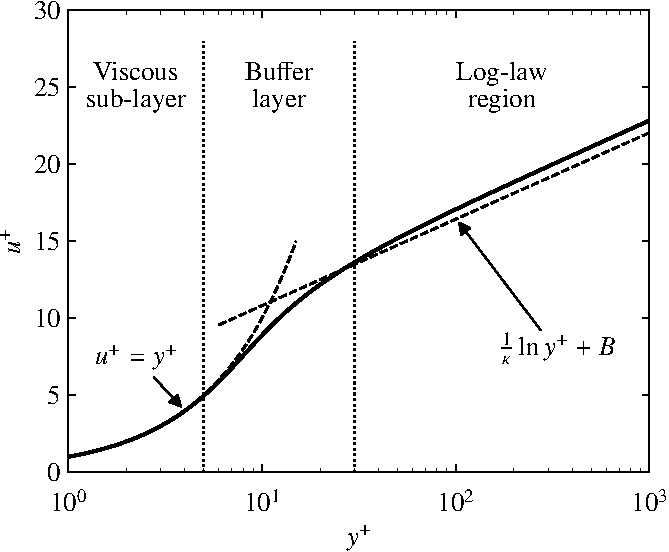
\includegraphics[height=0.45\linewidth]{Pictures/law_of_the_wall}
	\caption{Behaviour of the mean velocity profile in wall-bounded turbulent flows}
	\label{fig:law_of_the_wall}
\end{figure}

We have now algebraically defined Boussinesq's viscosity $\mu_\tau$ with another empirical parameter $\ell_m$. The specification of this mixing length typically relies on previous experimental data and is dependent on whether it is a jet, wake, wall boundary layer or another type of flow~\cite{andersonComputationalFluidMechanics2016}. Therefore, this model is considered to be incomplete, since it requires a previous understanding of the turbulent structures that are expected to be in the flow. 

\subsection{The Spalart-Allmaras Model}
Spalart and Allmaras~\cite{spalartOneequationTurbulenceModel1992} (SA) took an empirical approach, using arguments from dimensional analysis to develop a new model, which includes the resolution of an ad-hoc transport equation for a turbulence variable $\tilde \nu$. The model was initially developed for aerodynamics applications such as transonic flow over airfoils. Several nested versions are included in the original publication, which range from simple models for free shear flows to more complex derivations that can be applied to boundary layer flows. The general model is given by
\begin{eqBox}
\begin{equation}
    \frac{\partial \tilde{\nu}}{\partial t} 
    + v_i \frac{\partial\tilde\nu}{\partial x_i} 
    = c_{b1} (1-f_{t2}) \tilde S \tilde \nu
    + \frac{1}{\sigma} 
     \left[ \frac{\partial}{\partial x_j} \cdot \left((\nu + \tilde \nu)\frac{\partial\tilde\nu}{\partial x_j} \right) 
      + c_{b2}\left(\frac{\partial\tilde \nu}{\partial x_j} \right)^2\right]
    - \left[c_{w1}f_w - \frac{c_{b1}}{\kappa^2}f_{t2}\right],
    \label{eq:spalart_allmaras}
\end{equation}
\end{eqBox}
where $c$ and $f$ are empirical constants and functions of the turbulence model, which will be defined shortly along with the rest of the variables. Upon solving Equation~\ref{eq:spalart_allmaras}, we can compute the eddy viscosity $\mu_\tau$ from
\begin{equation}
    \mu_\tau=\rho \tilde \nu f_{v1},\quad \chi=\frac{\tilde \nu}{\nu},
    \label{eq:sa_eddyviscosity}
\end{equation}
where $\nu$ is the molecular kinematic viscosity. In addition,
\begin{equation}
    \tilde S \equiv S + \frac{\tilde \nu}{\kappa^2 d^2}f_{v2}~,\quad f_{v1}=\frac{\chi^3}{\chi^3+c_{v1}^3},\quad f_{v2}=1-\frac{\chi}{1+\chi f_{v1}},
\end{equation}
with $S$ the magnitude of the vorticity and $d$ the distance to the closest wall~\cite{spalartOneequationTurbulenceModel1992}. 
\begin{align}
    f_w&=g
    \left[\frac{1+c_{w3}^6}{g^6+c_{w3}^6}\right]^{1/6},& &r\equiv \min\left(\frac{\tilde\nu}{\tilde S \kappa^2 d^2},10\right). \\
    f_{t2}&=c_{t3} \exp \left[-c_{t4}\chi^2\right] & &g=\left[r+c_{w2}\left(r^6-r\right)\right].
\end{align}
Finally, the constants are given by 
\begin{align}
    &c_{b1} = 0.1355,& &c_{b2} =0.622,& &\sigma = 2/3,& &\kappa=0.41, \\
    &c_{w2} = 0.3,&    &c_{w3} =2,&     &c_{v1} = 7.1,&   &c_{t3}=1.2,  \\
    &c_{t4} = 0.5,&      &c_{w1} = \frac{c_{b1}}{\kappa^2} + \frac{1+c_{b2}}{\sigma}.
\end{align}
The implementation of this model allows us to remove the incomplete condition from the previously defined models. Wall and freestream boundary conditions are~\cite{rumseyRecentDevelopmentsTurbulence2015}
\begin{equation}
    \tilde \nu_{wall} = 0,\quad \tilde\nu_{\infty}=3 \nu_{\infty}:to:5\nu_{v_\infty},
\end{equation}
Now, by solving Equations~\ref{eq:spalart_allmaras} and~\ref{eq:sa_eddyviscosity}, we are able to give closure to the RANS equations. Since only one additional equation is required, the relative computational cost of this turbulence model makes it appealing. Given that this model was initially developed for aerospace applications, it is a popular choice for the prediction of aerodynamic loads at low to moderate angles of attack due to its relatively good resolution of boundary layer problems. 

Furthermore, the SA model is well-suited for applications using unstructured meshes. Despite its success in predicting aircraft performance, it has been found to unsuitable for flows that include jet-like free-shear regions and flows involving complex recirculation.
\subsection{The k-$\epsilon$ Model}
One of the most commonly used RANS models for the computation of turbulent flows is the $k-\epsilon$ model. It was originally developed to overcome the deficiencies of the mixing length model, such that no specification of flow-dependent properties are required. Instead, closure is achieved by resolving two transport equations for the turbulent kinetic energy $k$ and its rate of dissipation $\epsilon$. Hence this model is complete. Different versions of this model have been provided ~\cite{launderApplicationEnergydissipationModel1974, jonesPredictionLaminarizationTwoequation1972}. We describe the \textit{standard} $k-\epsilon$ model, as shown by~\cite{bardinaTurbulenceModelingValidation1997}. The relation between the eddy-viscosity and the two aforementioned turbulent quantities is given by
\begin{equation}
    \mu_\tau = c_\mu \rho k^2/\epsilon,
\end{equation}
where $c_\mu$ is a constant, which we define at the end of this section. Define the instantaneous kinetic energy to be the sum of the mean and the fluctuation component, such that
\begin{align}
    k(t) &= \overline{k} + k^\prime, \nonumber \\
         &= \frac{1}{2} \sum_{i=1}^d \overline{v}_i + \frac{1}{2}\sum_{i=1}^d \overline{v_i^\prime v_i^\prime}.
\end{align}
Hence, by multiplying each velocity component with their corresponding momentum equation in the appropriate direction, a PDE for the turbulent kinetic energy can be obtained. After performing Reynolds averaging and several algebraic operations, we can write
\begin{eqBox}
\begin{equation}
    \rho\frac{\partial k}{\partial t} + 
    \rho\overline v_j \frac{\partial k}{\partial x_j} 
    = \rho \hat \tau_{ij} \frac{\partial \overline v_i}{\partial x_j}
    - \rho\epsilon + \frac{\partial}{\partial x_j}\left[(\mu + \mu_\tau/\sigma_k)\frac{\partial k}{\partial x_j}\right].
\end{equation}
\end{eqBox}
The second component of this model is the dissipation rate $\epsilon$, for which the following transport equation was derived
\begin{eqBox}
\begin{equation}
    \rho \frac{\partial \epsilon}{\partial t}
    + \rho\overline v_j \frac{\partial\epsilon}{\partial x_j}
    = c_{\epsilon 1}\frac{\epsilon}{k}  \rho \hat \tau_{ij} \frac{\partial \overline v_i}{\partial x_j}
    - \rho c_{\epsilon2} \frac{\epsilon^2}{k} 
    + \frac{\partial}{\partial x_j} \left[(\mu + \mu_\tau/\sigma_\epsilon) \frac{\partial\epsilon}{\partial x_j}\right],
\end{equation}
\end{eqBox}
where the terms on the right-hand side refer to the diffusion, production and dissipation rates of $\epsilon$~\cite{andersonComputationalFluidMechanics2016}.
The constants are given by
\begin{align}
    & c_\mu = 0.09,   & & c_{\epsilon 1} = 1.44, & & c_{\epsilon 2} = 1.92, \\
    & \sigma_k = 1.0, & & \sigma_\epsilon = 1.3.  
\end{align}
The computational cost that comes from the computation of two transport equations can be significant. However, as previously mentioned, this model is one of the most commonly used in the CFD field, mostly for the modelling of free-shear layer flows with small to moderate pressure gradients. One of the pitfalls of this model, however, lies in the prediction of flows with large adverse pressure gradients, which cause the model to predict results inaccurately. This means that this model is often inaccurate for turbulent wall-bounded flows. Additional modifications, such as the introduction of wall functions, are necessary for such applications. Nevertheless, this model remains one of the simplest and most popular complete models.
\subsection{The k-$\omega$ Model}
The $k-\omega$ model is also a two-equation model, and along with the $k-\epsilon$ model, it is one of the most commonly used turbulence RANS models. Here, the equation for the turbulent kinetic energy is the same as in the $k-\epsilon$. The second transport equation, however, is derived for the specific dissipation rate, $\omega\equiv\epsilon/k$. The eddy viscosity is defined to be
\begin{equation}
    \mu_\tau = \rho\frac{k}{\tilde \omega}, \quad \tilde\omega= \max{\left[\omega, \frac{7}{8}\sqrt{2S_{ij}S_{ij}/\beta^*}\right]}.
\end{equation}
For the sake of completeness, we rewrite the PDE for the kinetic energy, now in terms of $\omega$
\begin{eqBox}
\begin{equation}
    \rho\frac{\partial k}{\partial t} + 
    \rho\overline v_j \frac{\partial k}{\partial x_j} 
    = \rho \hat \tau_{ij} \frac{\partial \overline v_i}{\partial x_j}
    - \rho\beta^* k\omega + \frac{\partial}{\partial x_j}\left[\left(\mu + \rho \sigma^* \frac{k}{\omega}\right)\frac{\partial k}{\partial x_j}\right].
\end{equation}
\end{eqBox}
The specific dissipation rate $\omega$ can be computed through~\cite{wilcox1998turbulence}
\begin{eqBox}
\begin{equation}
    \rho \frac{\partial \omega}{\partial t} + 
    \rho \overline v_j \frac{\partial \omega}{\partial x_j} 
    = \alpha \frac{\omega}{\kappa} \rho \hat \tau_{ij} \frac{\partial \overline v_i}{\partial x_j} 
    - \rho \beta \omega^2 
    + \rho \frac{\sigma_d}{\omega} \frac{\partial k}{\partial x_j} 
    \frac{\partial \omega}{\partial x_j} 
    + \frac{\partial}{\partial x_j} \left[\left(\mu + \rho\sigma\frac{k}{\omega}\right)\frac{\partial \omega}{\partial x_j}\right].
\end{equation}
\end{eqBox}
The closure coefficients and auxiliary relations are given by
\begin{align}
& \alpha= \frac{13}{25}, & & \beta = \beta_o f_\beta, & & \beta^* = \frac{9}{100}, \\
& \sigma = \frac{1}{2}, & & \sigma^* = \frac{3}{5}, & & \sigma_{do} = \frac{1}{8},
\end{align}
\[
    \sigma_{d} = 
\begin{cases}
    0,  &\dfrac{\partial k}{\partial x_j} \dfrac{\partial\omega}{\partial x_j}  \leq 0, \\
    \sigma_{do}, &\dfrac{\partial k}{\partial x_j} \dfrac{\partial\omega}{\partial x_j} > 0.
\end{cases}
\]
\begin{align}
    & \beta_0 = 0.0708, & & f_\beta = \frac{1+85\chi_\omega}{1+100\chi_\omega}, & & \chi_\omega\equiv \left|\frac{\Omega_{ij}\Omega_{jk}S_{ki}}{\left(\beta^* \omega\right)^3}\right|, \\
    & \epsilon = \beta^* \omega k, 
\end{align}
where $\Omega_{ij}$ is the mean-rotation tensor
\begin{equation}
    \Omega_{ij} = \frac{1}{2} \left( \frac{\partial \overline v_i}{\partial x_j}
    -\frac{\partial \overline v_j}{\partial x_i}\right),
\end{equation}
and $S_{ij}$ is the mean strain rate tensor, as described in Equation~\ref{eq:meanstrainrate}.

An advantage of this model is the relatively accurate resolution of near-wall interaction, and for flows with the presence of strong vorticity. This makes the $k-\omega$ approach suitable for applications such as turbomachinery. However, it was found to overpredict flow separation and to be highly sensitive to the freestream conditions. In addition, compared to the $k-\epsilon$ model, it is not an appropriate choice for free-shear flows. Further improvements to this model have been made to accommodate its shortcomings~\cite{wilcox1998turbulence}. Taking advantage of the relative accuracy of both the $k-\epsilon$ and $k-\omega$ models, combinations of these have been derived, such as the Shear Stress Transport (SST) model. We refer the reader to NASA's Turbulence Resource website for further details and additional turbulence models~\cite{rumseyRecentDevelopmentsTurbulence2015}.

\subsection{Summary of Turbulence Models}
We have introduced the basis of turbulence modelling using the RANS equations. As previously stated, these models are initially based on the Boussinesq approximation, where a constant coefficient referred to as the eddy viscosity, is used to model the behaviour of turbulence in a time-averaged sense. Further improvements, from the definition of a mixing length distance to the resolution of transport equations for turbulent quantities, have allowed the development of turbulence models to become applicable for real-world industrial applications. These models have been devised for specific applications and can also result in inaccurate results if not chosen appropriately. It is important to remember that these models are primarily limited by two approximations. First, the time-averaging of the Navier-Stokes equations removed the wide range of actual length scales characteristic of turbulent flows, which introduced the Reynolds stresses. Then, under the Boussinesq approximation, it was assumed that these Reynolds stresses could be reduced to a single unknown eddy viscosity, which is not always accurate. Then, this eddy viscosity is itself modelled using a turbulence model, which approximates the eddy viscosity to varying levels of realism.

To summarize the previous models, we present a table where we display the characteristic variables that define the model, the complete or incomplete condition according to~\cite{wilcox1998turbulence}, the number of equations to solve, and a general description including some common applications of each model.
\begin{table}[h]
    \centering
    \caption{Summary of popular turbulence models.}
\begin{tabular}{lp{0.17\linewidth}p{0.15\linewidth}p{0.35\linewidth}}
    \hline
    \textbf{Model} & \textbf{Variable(s)} & \textbf{Classification} & \textbf{Description} \\
    \hline
    ML           & A mixing length $\ell_m$        & Incomplete, algebraic model    & An empirical mixing length is used to compute the eddy viscosity. This model was developed in a "rough" sense. Value of $\ell_m$ depends on the type of flow. \\
    \hline
    SA           & Turbulent quantity proportional to the viscosity $\tilde\nu$     & Complete, one-equation model    & Resolution of a transport equation for a turbulent quantity, specifically a viscosity-like parameter. Computationally efficient since only a single transport equation is added. Applicable to determine aerodynamic loads at moderate angles of attack.             \\
    \hline
    $k-\epsilon$ & Kinetic energy and rate of dissipation, $k$, $\epsilon$ & Complete, two-equation model   & Two transport equations are added, one for the turbulent kinetic energy and the other for its rate of dissipation. Applicable to free-shear layer flows. Gives inaccurate results for flows with large adverse pressure gradients.\\
    \hline
    $k-\omega$   & Kinetic energy and specific dissipation $k$, $\omega$   & Complete, two-equation model    & Requires the computation of the kinetic energy and specific dissipation rate transport equations. The model works well across the boundary layer of wall turbulent flows, hence widely used in the aerospace field. Inaccurate for free-shear flows.\\
    \hline
\end{tabular}
\end{table}
More complex models can be found in the literature. These include not only additional eddy-viscosity models but also other types of models such as Large Eddy Simulation (LES), which do not require a time-averaged RANS system of equations. For further references, refer to the NASA Turbulence Resource database~\cite{rumseyRecentDevelopmentsTurbulence2015}.
\chapter{Boundary Conditions}
\section{Wall Boundaries}
\subsection{Wall-Bounded Turbulence}
In order to properly enforce the wall boundary conditions, it is necessary to have a computational mesh that is sufficiently fine in this region. To better understand the physics of the flow in this region, we will reconsider the incompressible RANS momentum equations of the form
\begin{equation}
    \rho \frac{\partial \overline{v_i}}{\partial t} 
    + \rho  \frac{\partial}{\partial x_j} \left(\overline{v_j}\overline{v_i}\right)
    =- \frac{\partial \overline{p}}{\partial x_i} 
    + \frac{\partial}{\partial x_j} \left(\overline\tau_{ji} - \rho \overline{v_j^\prime v_i^\prime}\right).
\end{equation}
Assuming that a full time average has been computed, the temporal derivative can be ommitted
\begin{equation}
    \rho  \frac{\partial}{\partial x_j} \left(\overline{v_j}\overline{v_i}\right)
    =- \frac{\partial \overline{p}}{\partial x_i} 
    + \frac{\partial}{\partial x_j} \left(\overline\tau_{ji} - \rho \overline{v_j^\prime v_i^\prime}\right).
\end{equation}
Furthermore, if we assume that the pressure gradient term is negligible and that the streamwise velocity varies primarily in the vertical direction, then the vertical momentum equation yields
\begin{equation}
	\label{eqn:3nsi2039}
	\nu \frac{\partial \overline{u}}{\partial y} - \overline{u^\prime v^\prime} = \nu \Eval{\frac{\partial \overline{u}}{\partial y}}{y=0}{},
\end{equation}
after integration. This implies that the rate of streamwise momentum transport away from the wall is constant through the boundary layer, and that it is equal to the viscous stress that the wall applies to the fluid. Furthermore, there are two mechanisms that are responsible for transporting this momentum in the boundary layer. The first term, $\nu \partial \overline{u}/\partial y$, is simply the steady viscous stress that applies due to the shear in the fluid moving up the boundary layer. In contrast, $-\overline{u^\prime v^\prime}$, are the Reynolds stresses. These are responsible for transporting momentum through the boundary layer by physically moving it. Upward velocity fluctuations tend to move slow-moving fluid near the wall up in the boundary layer. In contrast, downward velocity fluctuations tend to move fast-moving fluid near the free stream down in the boundary layer, transporting momentum. Based on physical observations, the boundary layer is typically divided into three distinct regions.
\subsubsection{The Inner Layer}
The inner layer is the region very close to the wall boundary. The no-slip boundary condition that forces the velocity towards zero and, as previously discussed, the fluctuating velocity components also vanish here. Hence, in the inner layer, Equation \ref{eqn:3nsi2039} reduces to
\begin{equation}
	\label{eqn:3nsi2039}
	\nu \frac{\partial \overline{u}}{\partial y} = \nu \Eval{\frac{\partial \overline{u}}{\partial y}}{y=0}{}.
\end{equation}
In this region of the boundary layer, momentum is transported almost entirely by viscous effects.
\subsubsection{The Outer Layer}
In the outer regions of the boundary layer, the mean velocity gradient becomes negligible. Hence, the viscous effects can be omitted and Equation \ref{eqn:3nsi2039} reduces to
\begin{equation}
	\label{eqn:3nsi2039}
	 - \overline{u^\prime v^\prime} = \nu \Eval{\frac{\partial \overline{u}}{\partial y}}{y=0}{},
\end{equation}
Hence, in this region of the boundary layer, momentum is transported almost entirely by turbulent fluctuations. Classical experiments have shown this is well-approximated via a log-law, as shown in Figure~\ref{fig:law_of_the_wall}.
\subsubsection{The Buffer Layer}
The buffer layer is simply the region between the inner and outer layers. Neither the viscous nor the Reynolds stress terms dominate here, and hence Equation \ref{eqn:3nsi2039} remains unchanged.

In order to better understand the behaviour of a boundary layer, we will first non-dimensionalize it using parameters from within the boundary layer, resulting in the dimensionless {\it wall-units}. Starting with the shear stress at the wall and the density, we obtain the friction velocity
\begin{equation}
	u^{\tau} = \sqrt{\frac{\tau_w}{\rho}}.
\end{equation}
From this, we can now define a dimensionless height
\begin{equation}
	y^+ = \frac{y u^{\tau}}{\nu},
\end{equation} 
typically called ``y plus'', and a dimensionless velocity
\begin{equation}
	u^+ = u/u^{\tau},
\end{equation} 
typically called ``u plus''. A plot of a standard boundary layer profile, including these three regions, is given in Figure \ref{fig:law_of_the_wall}. This shows that, interestingly, the velocity profile far from the wall boundary can be well-approximated using a logarithmic profile.
